\documentclass[a4paper]{article}
\usepackage{fancyhdr}
\usepackage{lastpage}
\usepackage{graphicx}
\usepackage{twocolceurws}
\usepackage{amsmath}

% Configure the fancyhdr package
\pagestyle{fancy}
\fancyhf{}
\fancyfoot[C]{Page \thepage\ of \pageref{LastPage}}  % Centered footer with page number


\title{Unsupervised Learning: Anomaly Detection in Hypothyroidism dataset}

\institution{University of Milan-Bicocca}

\author{
\textbf{Andrea Palmieri} \\  a.palmieri13@campus.unimib.it \\ Matricula  921785
\and
\textbf{Andrea Yachaya} \\ a.yachaya@campus.unimib.it \\ Matricula 913721
}

\begin{document}
\maketitle

\begin{abstract}
\textbf{The purpose of this report is to present a comprehensive overview of the methodologies employed for analyzing a dataset and detecting anomalous observations. These methodologies were applied to the Hypothyroidism dataset, which contains records of patients diagnosed with Hypothyroidism, commonly referred to as underactive thyroid disease. This condition arises when the thyroid gland fails to produce sufficient thyroid hormones to meet the body's requirements.}
\end{abstract}


\section{Introduction}

Anomaly detection is a crucial aspect of data analysis, especially in healthcare, where identifying rare or unusual cases can significantly impact patient outcomes. This report focuses on anomaly detection within the Hypothyroidism dataset, which consists of 7,200 observations with 15 binary columns and 6 continuous columns. The primary goal of this study was to identify abnormal patterns or anomalies that may indicate potential health issues or data quality problems and compute a probability score of an observation being anomaly.


\section{Dataset Preprocessing}
To prepare the dataset for analysis, several preprocessing steps were undertaken. First, the continuous features were standardized to prevent any single feature from disproportionately influencing the results, using the following equation:
\begin{equation}
Z = \frac{x - \mu}{\sigma}
\end{equation}
where \( Z \) is the standardized value, \( x \) is the original value, \( \mu \) is the mean of the feature, and \( \sigma \) is the standard deviation of the feature.
\\Second, the binary features were converted to object data types. Given that these features are binary, one-hot encoding was not necessary, as each feature already represents a distinct categorical variable.
\\Finally, the original classes of each sample in the dataset are not provided. Consequently, our project focuses on unsupervised learning techniques to identify anomalies without relying on class labels.

\section{Dimensionality Reduction}

\subsection{Anomaly detection using PCA}
We have prioritized the exclusion of Principal Component Analysis (PCA) for anomaly detection due to its inherent methodology. PCA operates by transforming the original dataset into a series of linearly uncorrelated components, ordered based on the variance they explain. This procedure entails computations involving the covariance matrix, as well as the determination of eigenvalues and eigenvectors. These mathematical operations necessitate numerical data, as covariance, eigenvalues, and eigenvectors are concepts that do not directly apply to categorical data. Given that our dataset comprises mixed data types, including categorical variables, we have determined that PCA is unsuitable for our purposes, as it is unable to effectively handle non-continuous features.

\subsection{FAMD}
To overcome the limitations of PCA, we employed Factor Analysis of Mixed Data (FAMD) as a dimensionality reduction technique. FAMD is a variant of PCA that can handle mixed data types, including categorical and continuous variables, making it particularly useful for our dataset. However, FAMD cannot be used for anomaly detection because the original features cannot be reconstructed from the FAMD coordinates.
Instead, by applying FAMD we aim to reduce the dimensionality of the data and identify the most informative features that capture the underlying structure of the data. This will enable us to visualize the data in a lower-dimensional space, facilitating the identification of patterns and anomalies. We expect FAMD to provide a more comprehensive representation of our dataset, capturing the relationships between the continuous and categorical variables. The resulting lower-dimensional representation will be used to visualize our clustering results and gain a better understanding of how the dataset is organized.
In the next sections, we will discuss the clustering algorithms used to identify anomalies in the dataset.

\section{Distance Based Clustering}
The first category of approaches implemented were about distance-based clustering algorithms. These methods group similar data points into clusters based on some measure of distance or similarity. These algorithms rely on the concept of distance (or dissimilarity) between data points to form clusters where points within the same cluster are more similar (closer) to each other than to those in other clusters. Since we are dealing with a dataset containing mixed data-type, euclidean distance operates under the assumption of continuous, numerical data. It calculates the straight-line distance between points in a multi-dimensional space, which works well when dealing with numeric attributes that represent continuous quantities, such as temperature or length. Moreover, in high-dimensional spaces, Euclidean distance can become less meaningful. This is often referred to as the "curse of dimensionality." As the number of dimensions increases, the distance between points becomes more similar, and it becomes difficult to differentiate between points. This phenomenon can lead to poor performance in clustering and classification tasks. \newline
To address this problems, we employed the use of a different distance metric: the Gower distance

\subsection{Gower distance}
The Gower distance is a metric used to calculate the dissimilarity or distance between two points in a dataset, particularly useful in situations where traditional distance metrics like Euclidean distance may not be appropriate due to the nature of the data. Gower distance $d_{i,j}$ between two data points i and j in a dataset with p variables can be calculated using the following formula:
\begin{equation}
    d_{i,j} = \frac{ \sum_{k=1}^{p} w_k \cdot \delta_k(x_{ik}, x_{jk}) }{ \sum_{k=1}^p w_k }
\end{equation}
where:
\begin{itemize}
    \item $w_k$ is the weight for variable k
    \item $\delta_k(x_{ik}, x_{jk})$ is the dissimilarity measure for variable k between data points $i$ and $j$
\end{itemize}
For numerical variables, the dissimilarity $ \delta_k(x_{ik}, x_{jk}) $ is calculated using the absolute difference between the normalized values of the feature:
\begin{equation}
    \delta_k(x_{ik}, x_{jk}) = \frac{|x_{ik} - x_{jk}|}{\max(x_k) - \min(x_k)}
\end{equation}
where:
- $ x_{ik} $ and $ x_{jk} $ are the values of the $ k $-th feature for observations $ i $ and $ j $,
- $ \max(x_k) $ and $ \min(x_k) $ are the maximum and minimum values of the $ k $-th feature across all observations. \newline
For categorical variables, the dissimilarity $ \delta_k(x_{ik}, x_{jk}) $ is calculated using a simple matching approach:
\begin{equation}
    \delta_k(x_{ik}, x_{jk}) = 
    \begin{cases}
       0 & \text{if } x_{ik} = x_{jk} \\
       1 & \text{if } x_{ik} \ne x_{jk}
    \end{cases}
\end{equation}
where $ x_{ik} $ and $ x_{jk} $ are the values of the $ k $-th feature for observations $ i $ and $ j $. \newline
In our specific case we imposed all the weights equals to each other since we didn't have any domain-specific knowledge about the dataset to sensibly impose a different weight to one or more variables. The proximity matrix created using Gower distance, which will be used by clustering methods we developed during the project, is shown in figure [\ref{fig:ProximityDistanceGower}].

\begin{figure}
    \centering
    \includegraphics[width=0.45\textwidth]{images/ProximityDistanceGower.png}
    \caption{Proximity distance matrix using gower distance}
    \label{fig:ProximityDistanceGower}
\end{figure}

\subsection{Hierarchical Clustering}
Hierarchical clustering is a powerful technique that produces nested clusters, which can be visualized as a dendrogram. This method is particularly useful for understanding the hierarchical relationships between clusters. In agglomerative hierarchical clustering, there are several methods to compute inter-cluster proximity, each with its own advantages and disadvantages. These methods include minimum (single linkage), maximum (complete linkage), average (UPGMA), centroids-based methods, and Ward's method, which minimizes the sum of squared errors within clusters.
\\Ward's method tends to create globular clusters, making it a good candidate for initializing K-means clustering. However, Ward's method and centroid-based methods require the use of Euclidean distances and are not suitable for non-Euclidean distance metrics like the Gower distance.
\\For this reason hierarchical clustering was performed with the following linkage methods: \textit{complete} and \textit{average}. These methods do not require Euclidean distances and can work directly with the Gower distance matrix.

\begin{figure}
    \centering
    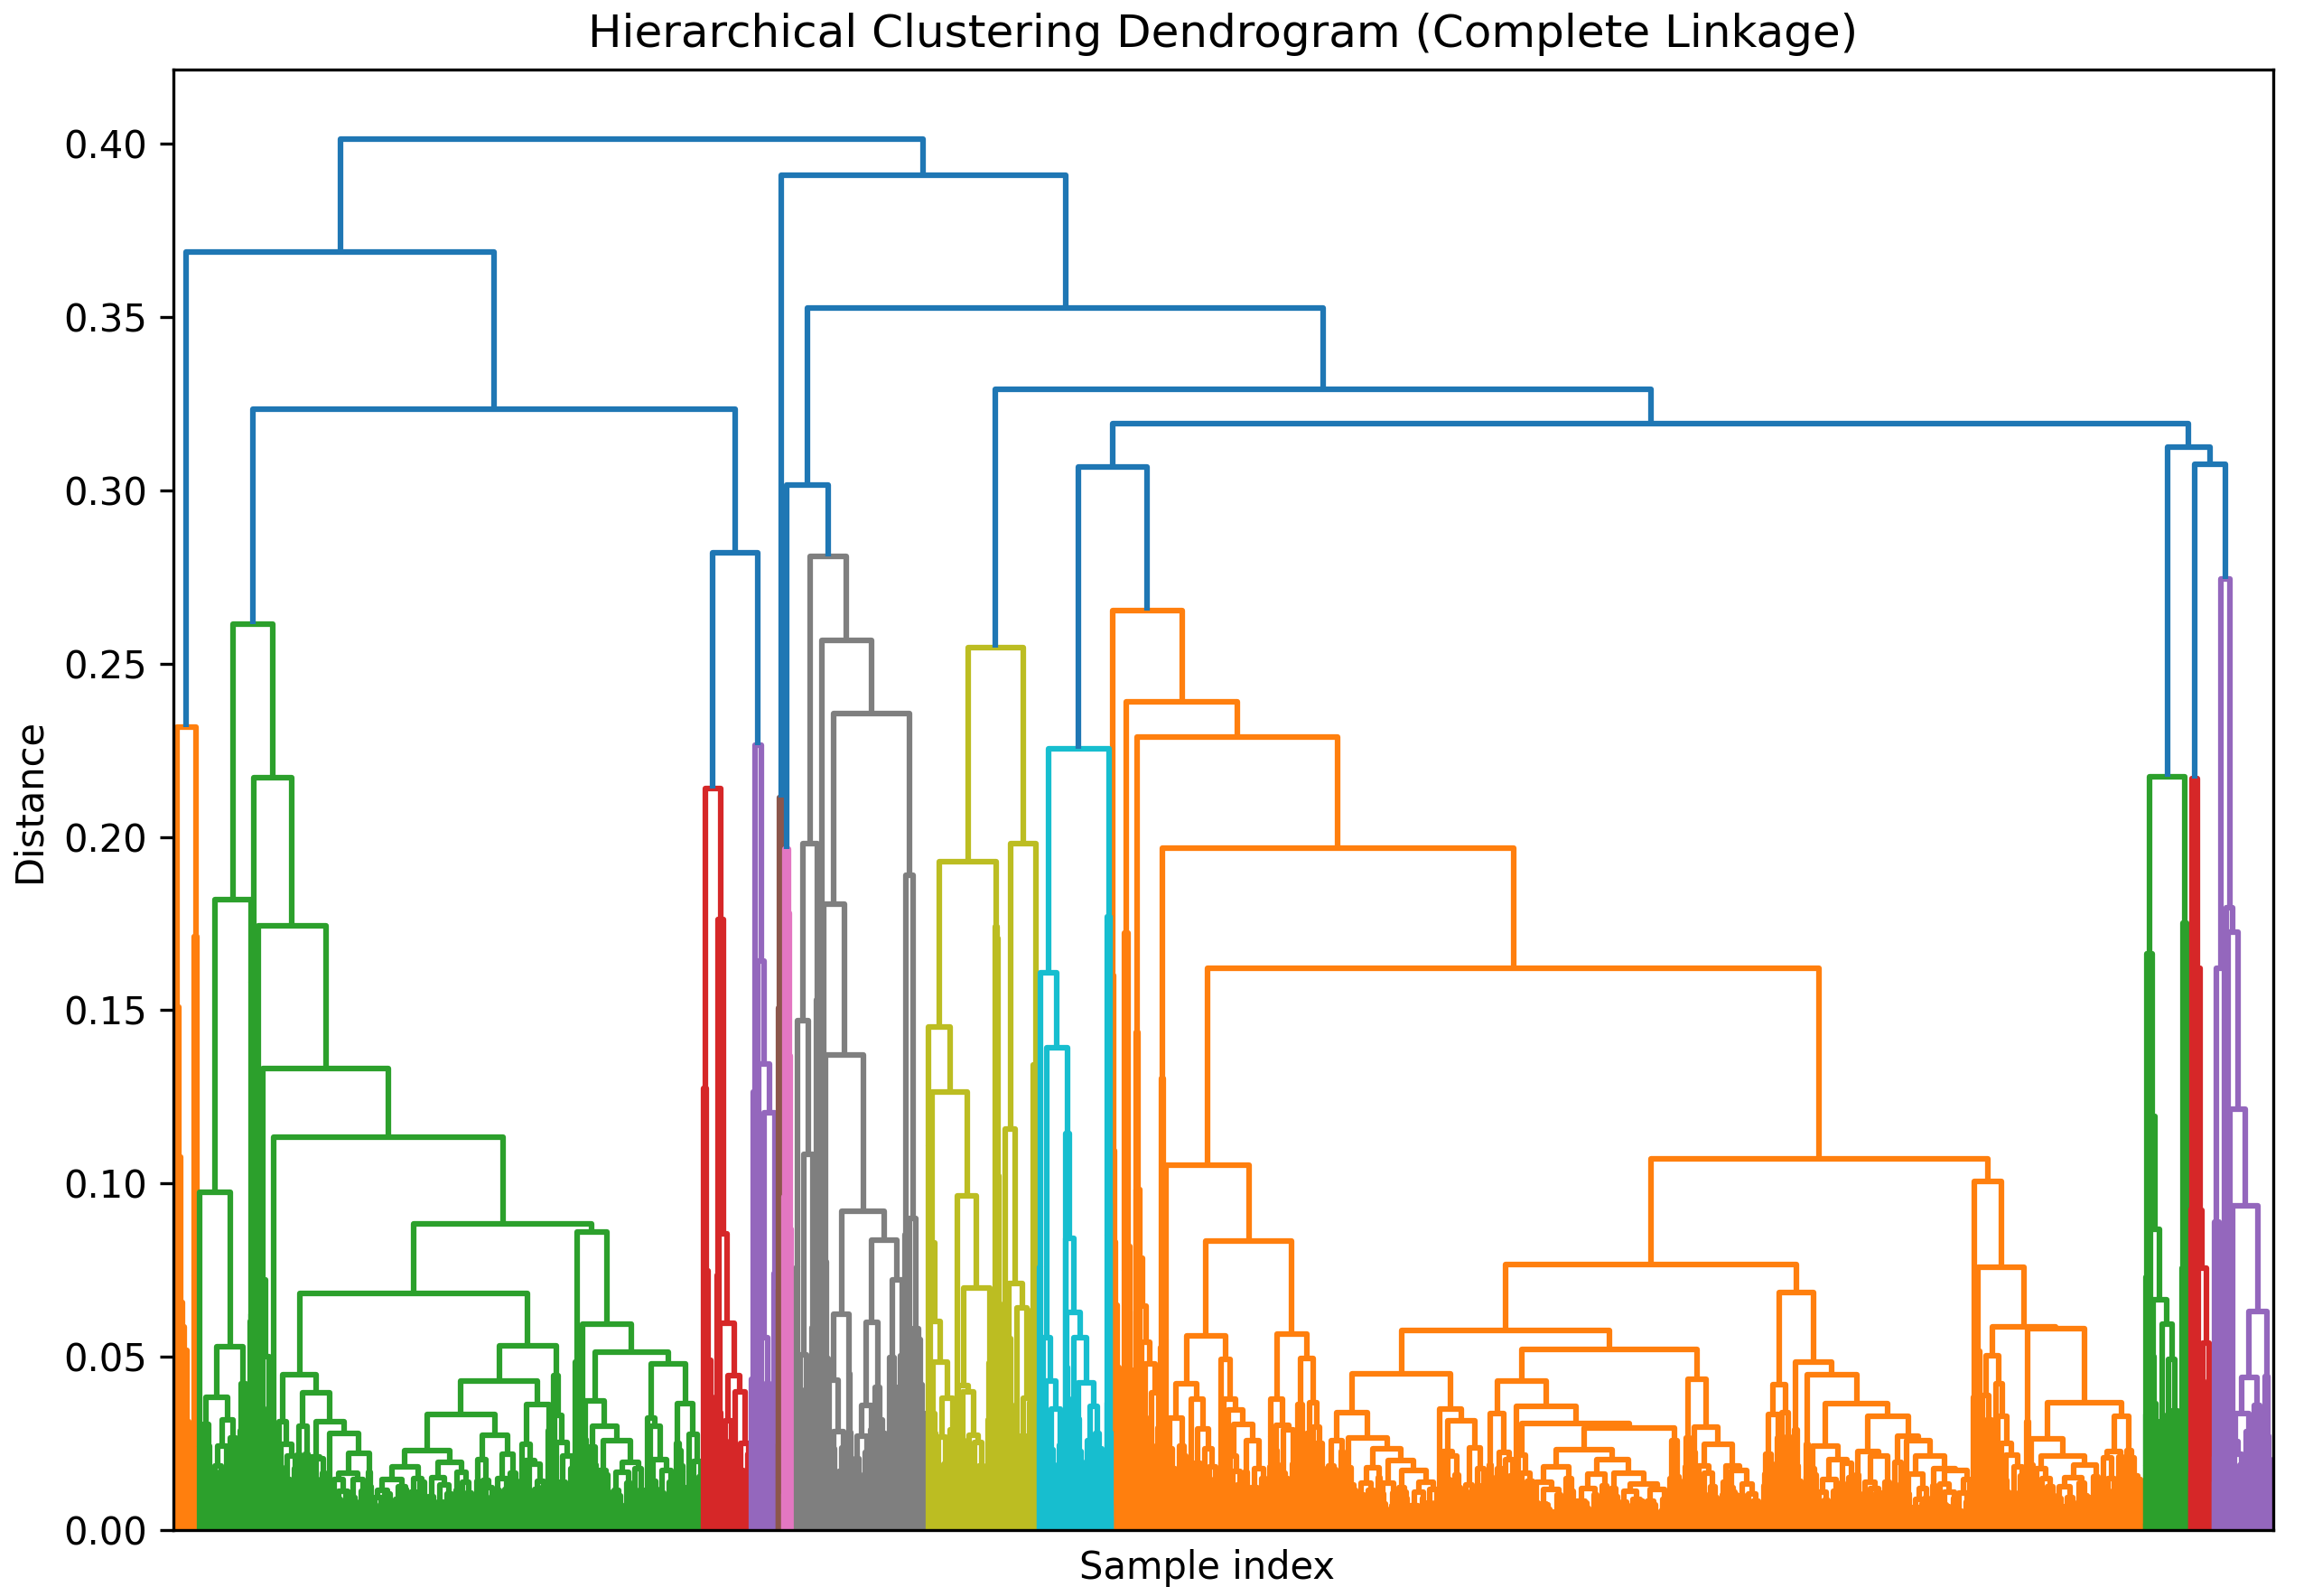
\includegraphics[width=0.45\textwidth]{images/dendrogram_complete_linkage.png}
    \caption{Dendrogram with \textit{complete} as linkage method}
    \label{fig:dendrogram_complete_linkage}
\end{figure}

\begin{figure}
    \centering
    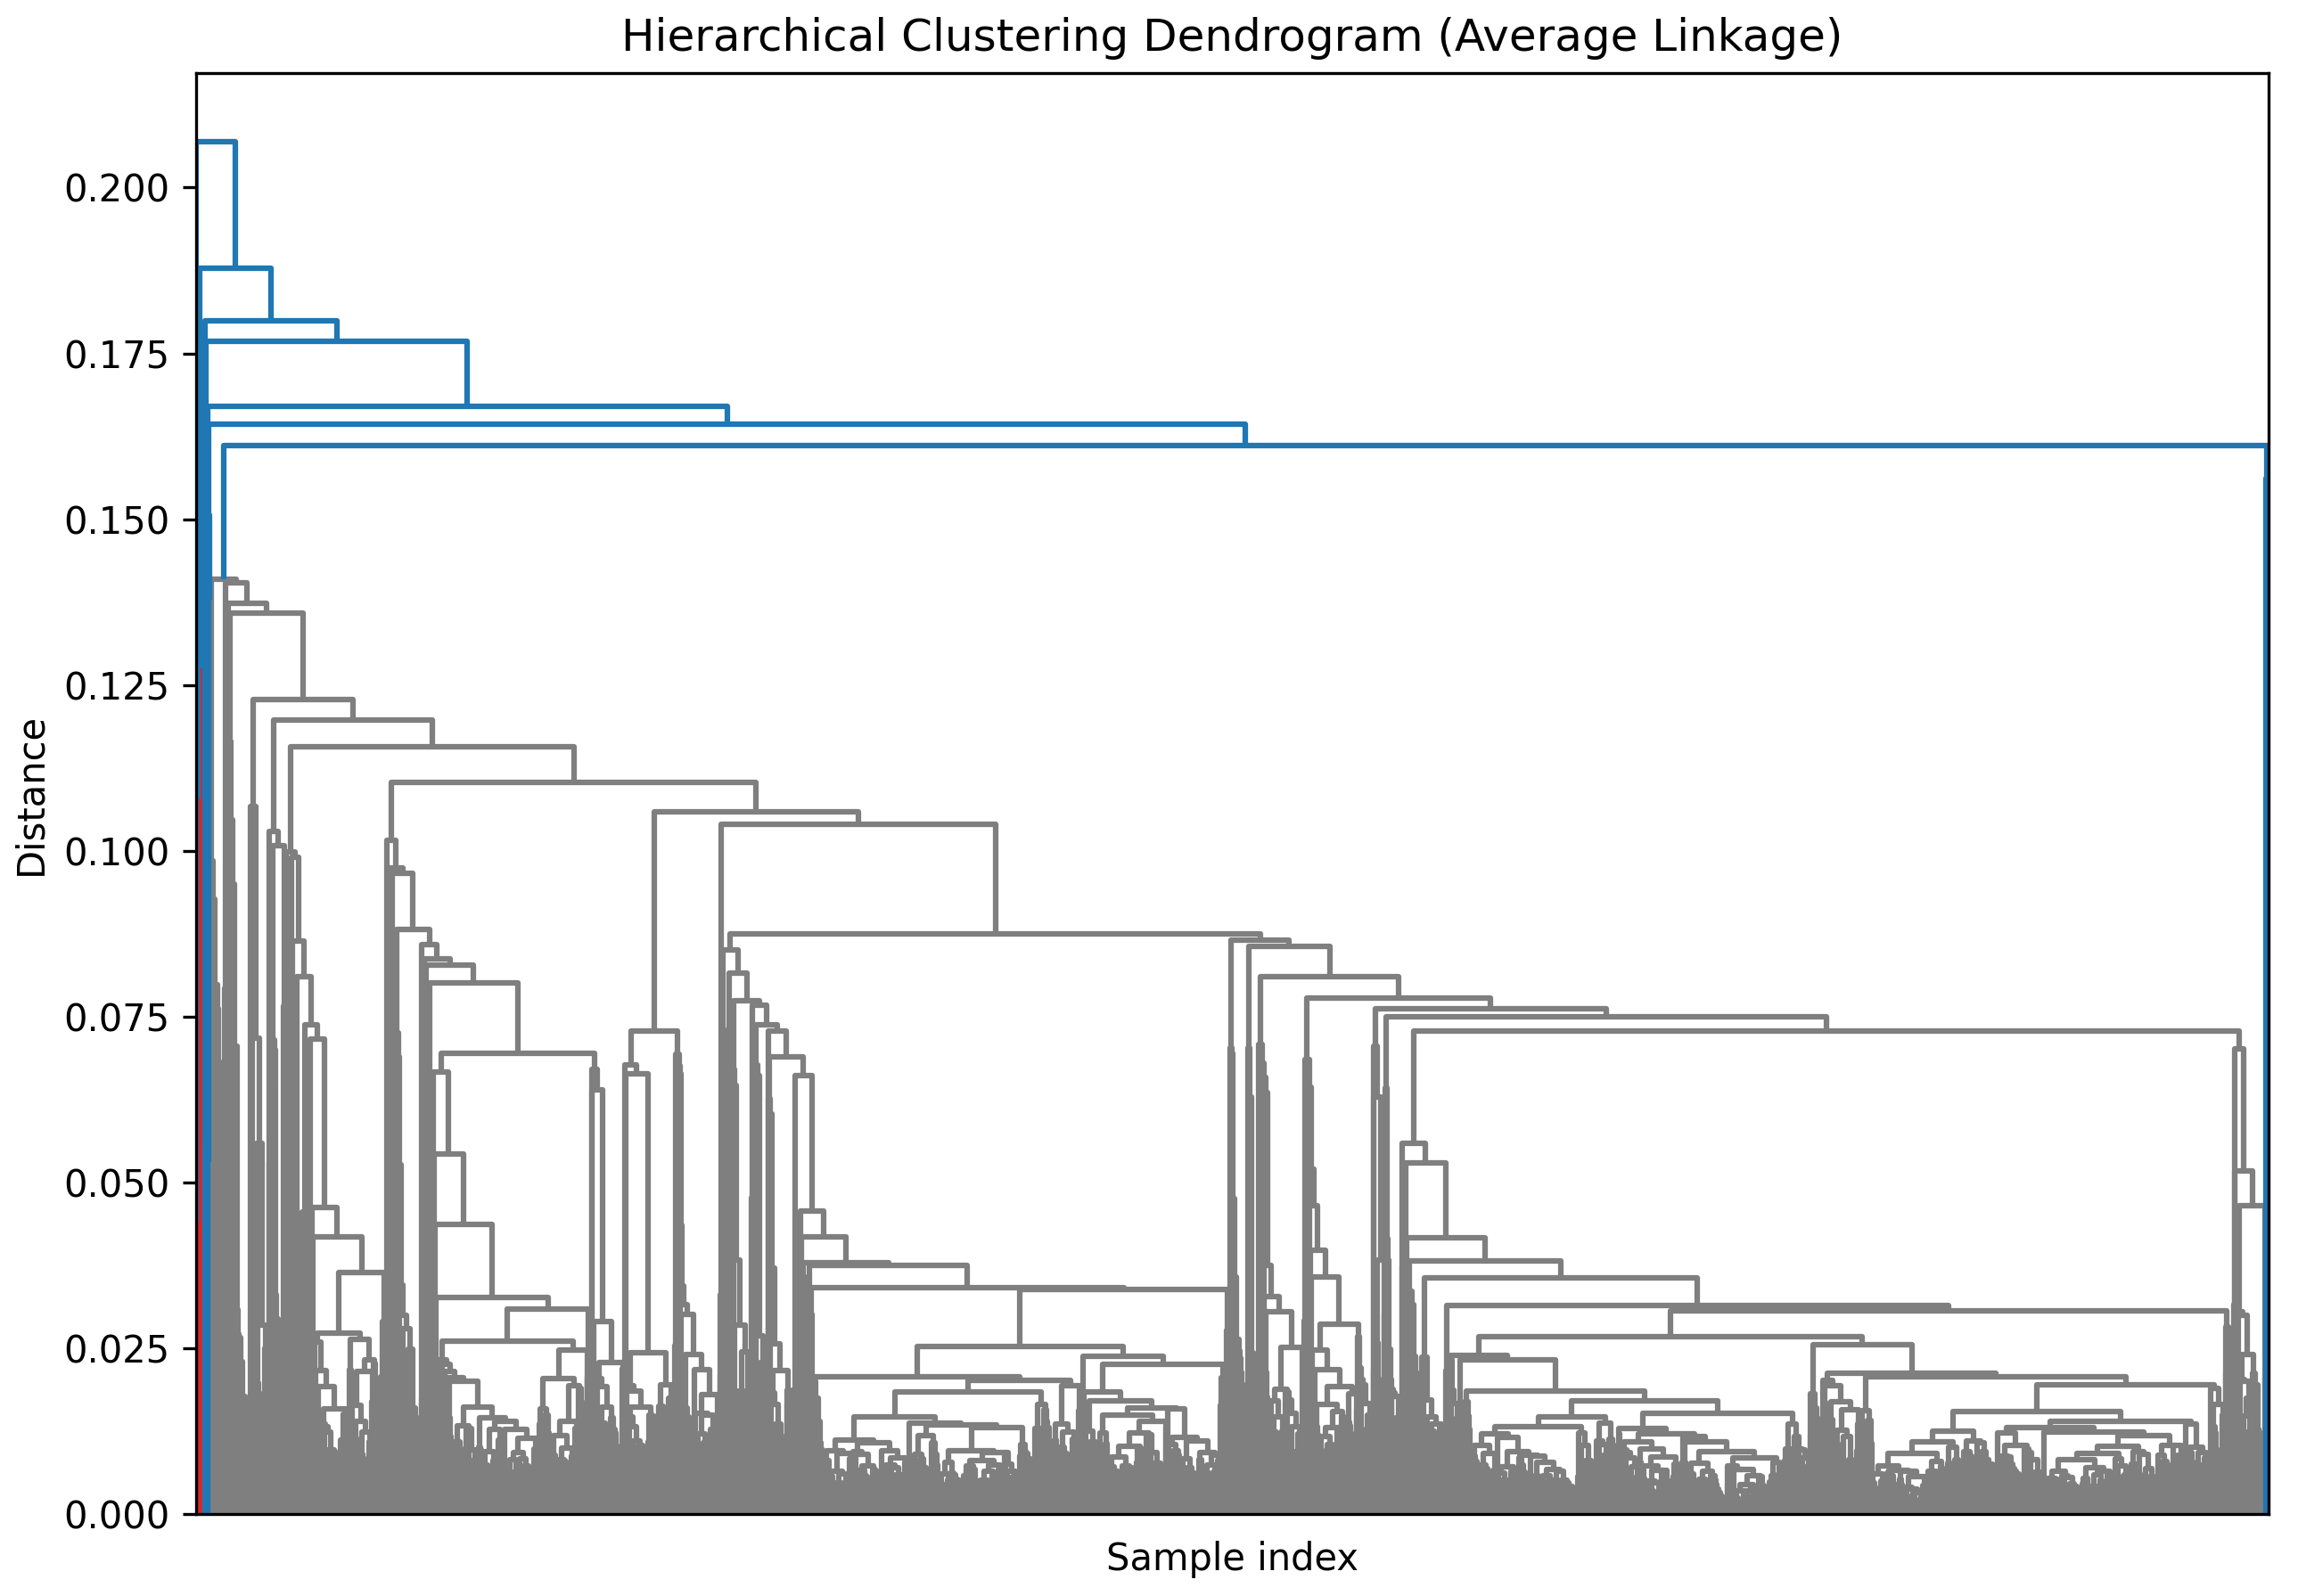
\includegraphics[width=0.45\textwidth]{images/dendrogram_average_linkage.png}
    \caption{Dendrogram of with \textit{average} as linkage method}
    \label{fig:dendrogram_average_linkage}
\end{figure}

\subsubsection{Comparison of Linkage Methods and Analysis}
The complete linkage method tries to minimize the maximum distance between points within each cluster, leading to the formation of compact clusters with small diameters. However, this method is susceptible to noise and anomalies, as a single anomaly can significantly increase the distance between clusters. The dendrogram in Figure [\ref{fig:dendrogram_complete_linkage}] shows a highly branched structure with many small clusters, indicating that the complete linkage method has formed numerous small, tight clusters.
On the other hand, the average linkage method defines the distance between two clusters as the average distance between all pairs of points, where one point is from each cluster. This method tends to produce clusters with roughly equal variance and is less susceptible to noise and anomalies compared to the complete linkage method. The dendrogram in Figure [\ref{fig:dendrogram_average_linkage}] shows a more balanced structure with fewer branches and larger clusters. The average linkage method has formed fewer but larger clusters, with a more gradual increase in the distance between clusters as the clusters merge.

\begin{figure}
    \centering
    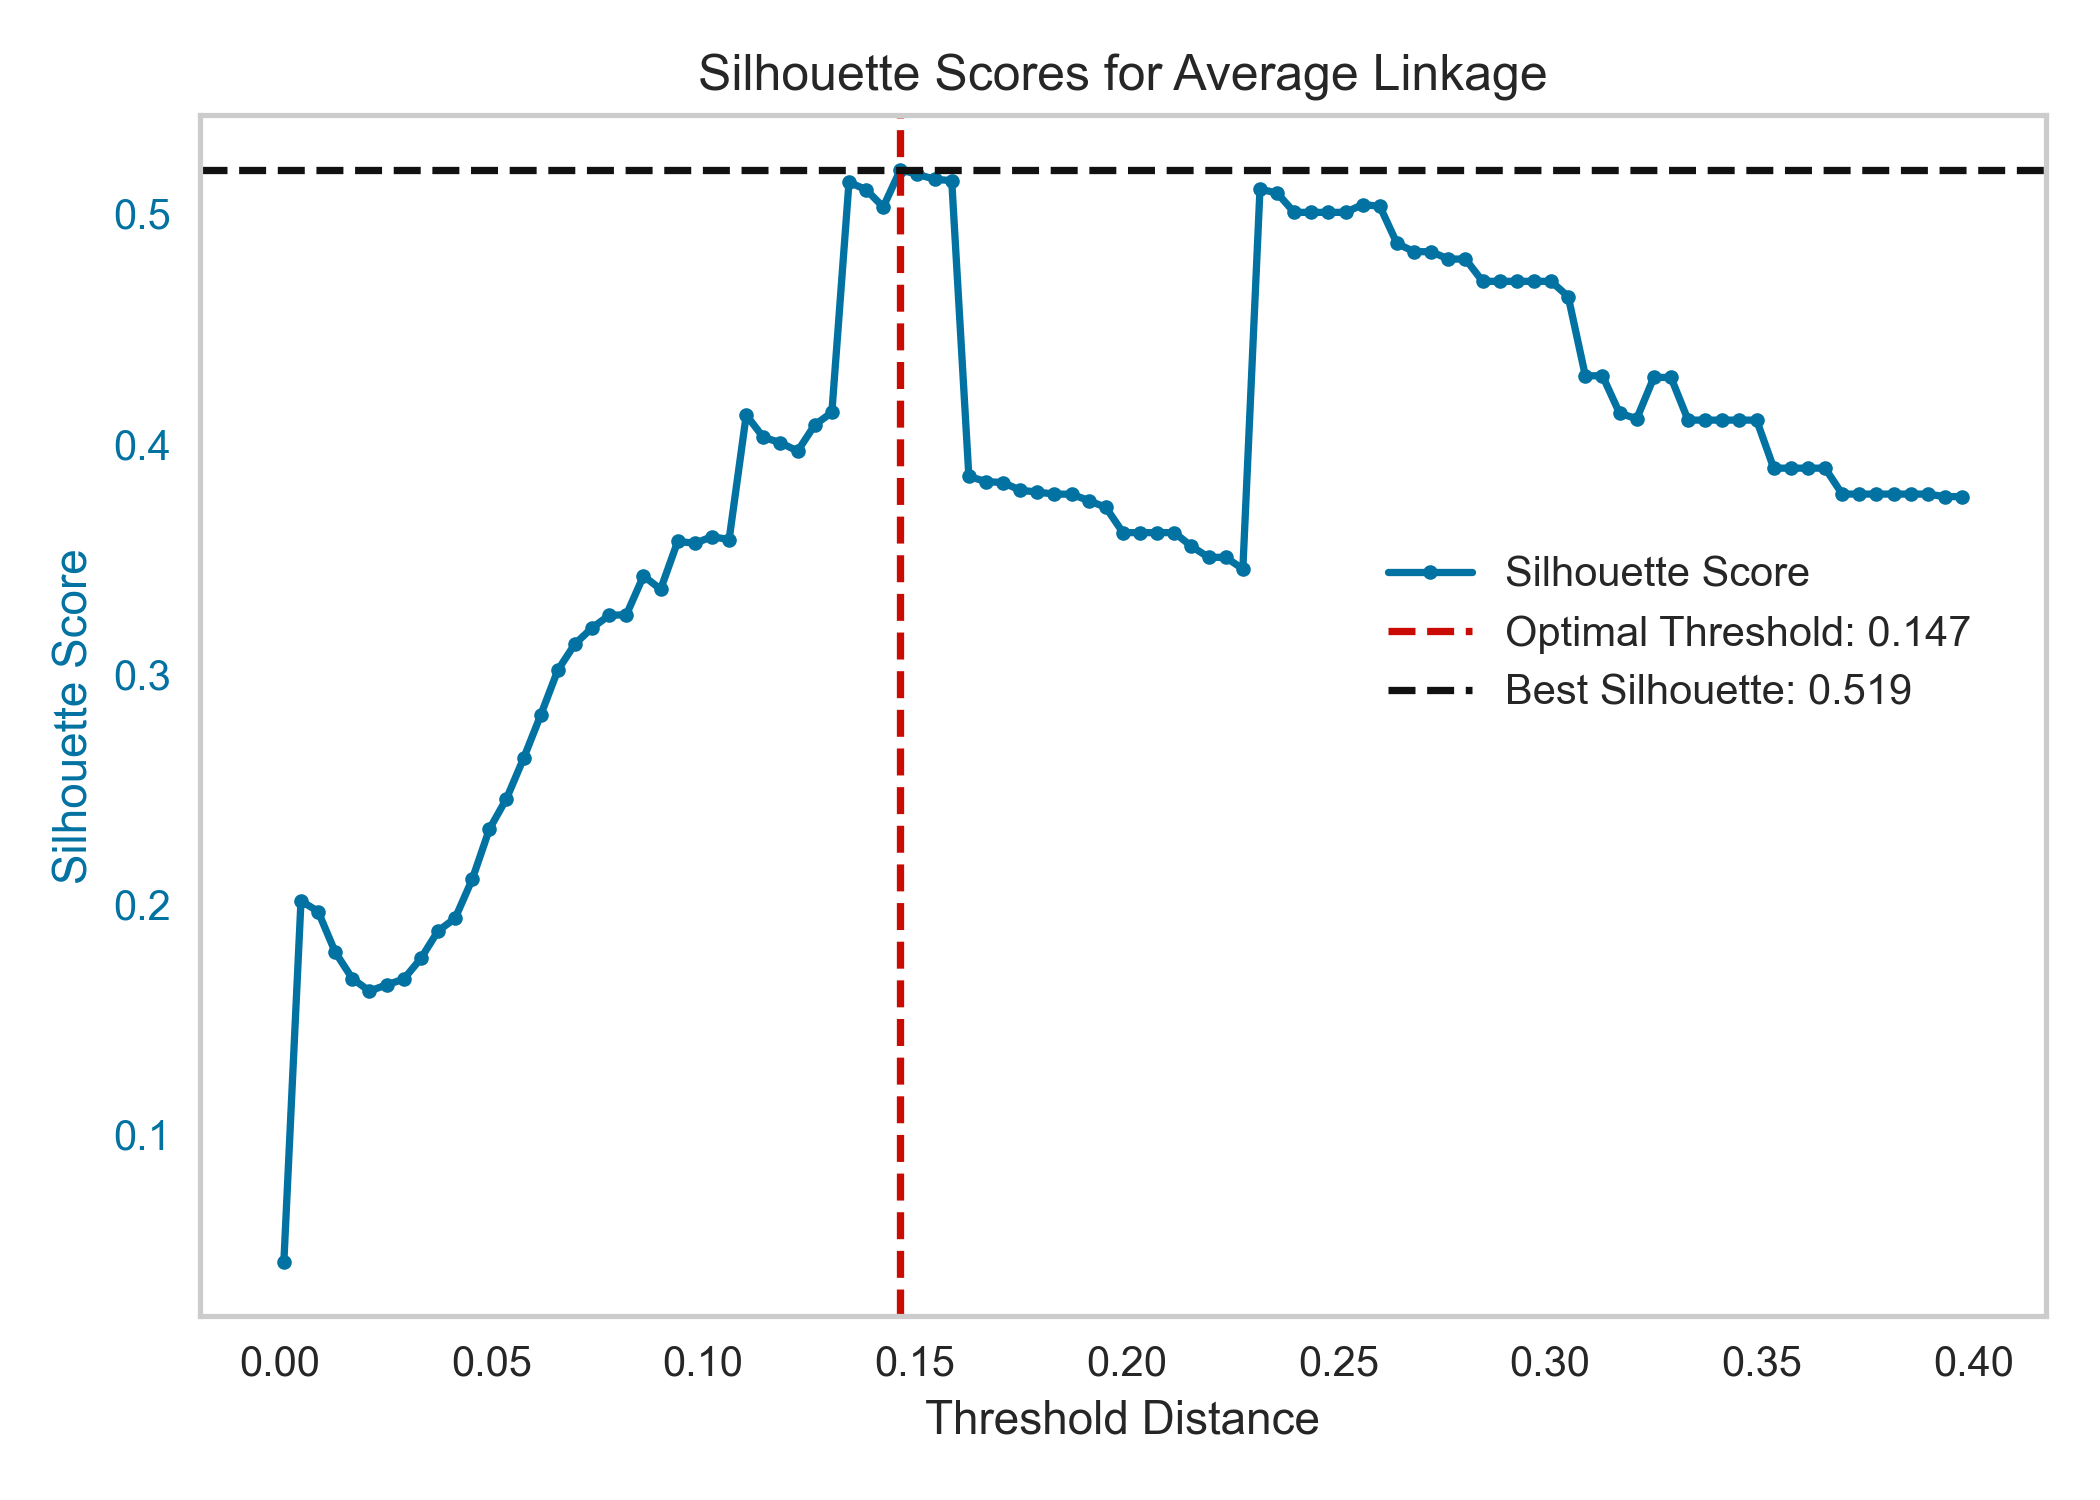
\includegraphics[width=0.45\textwidth]{images/silhouette_score_complete_linkage.png}
    \caption{Silhouette score and number of anomalies with \textit{complete} as linkage method at varying distance threshold. Optimal distance 0.147 with silhouette 0.519.}
    \label{fig:silhouette_score_complete_linkage}
\end{figure}

\begin{figure}
    \centering
    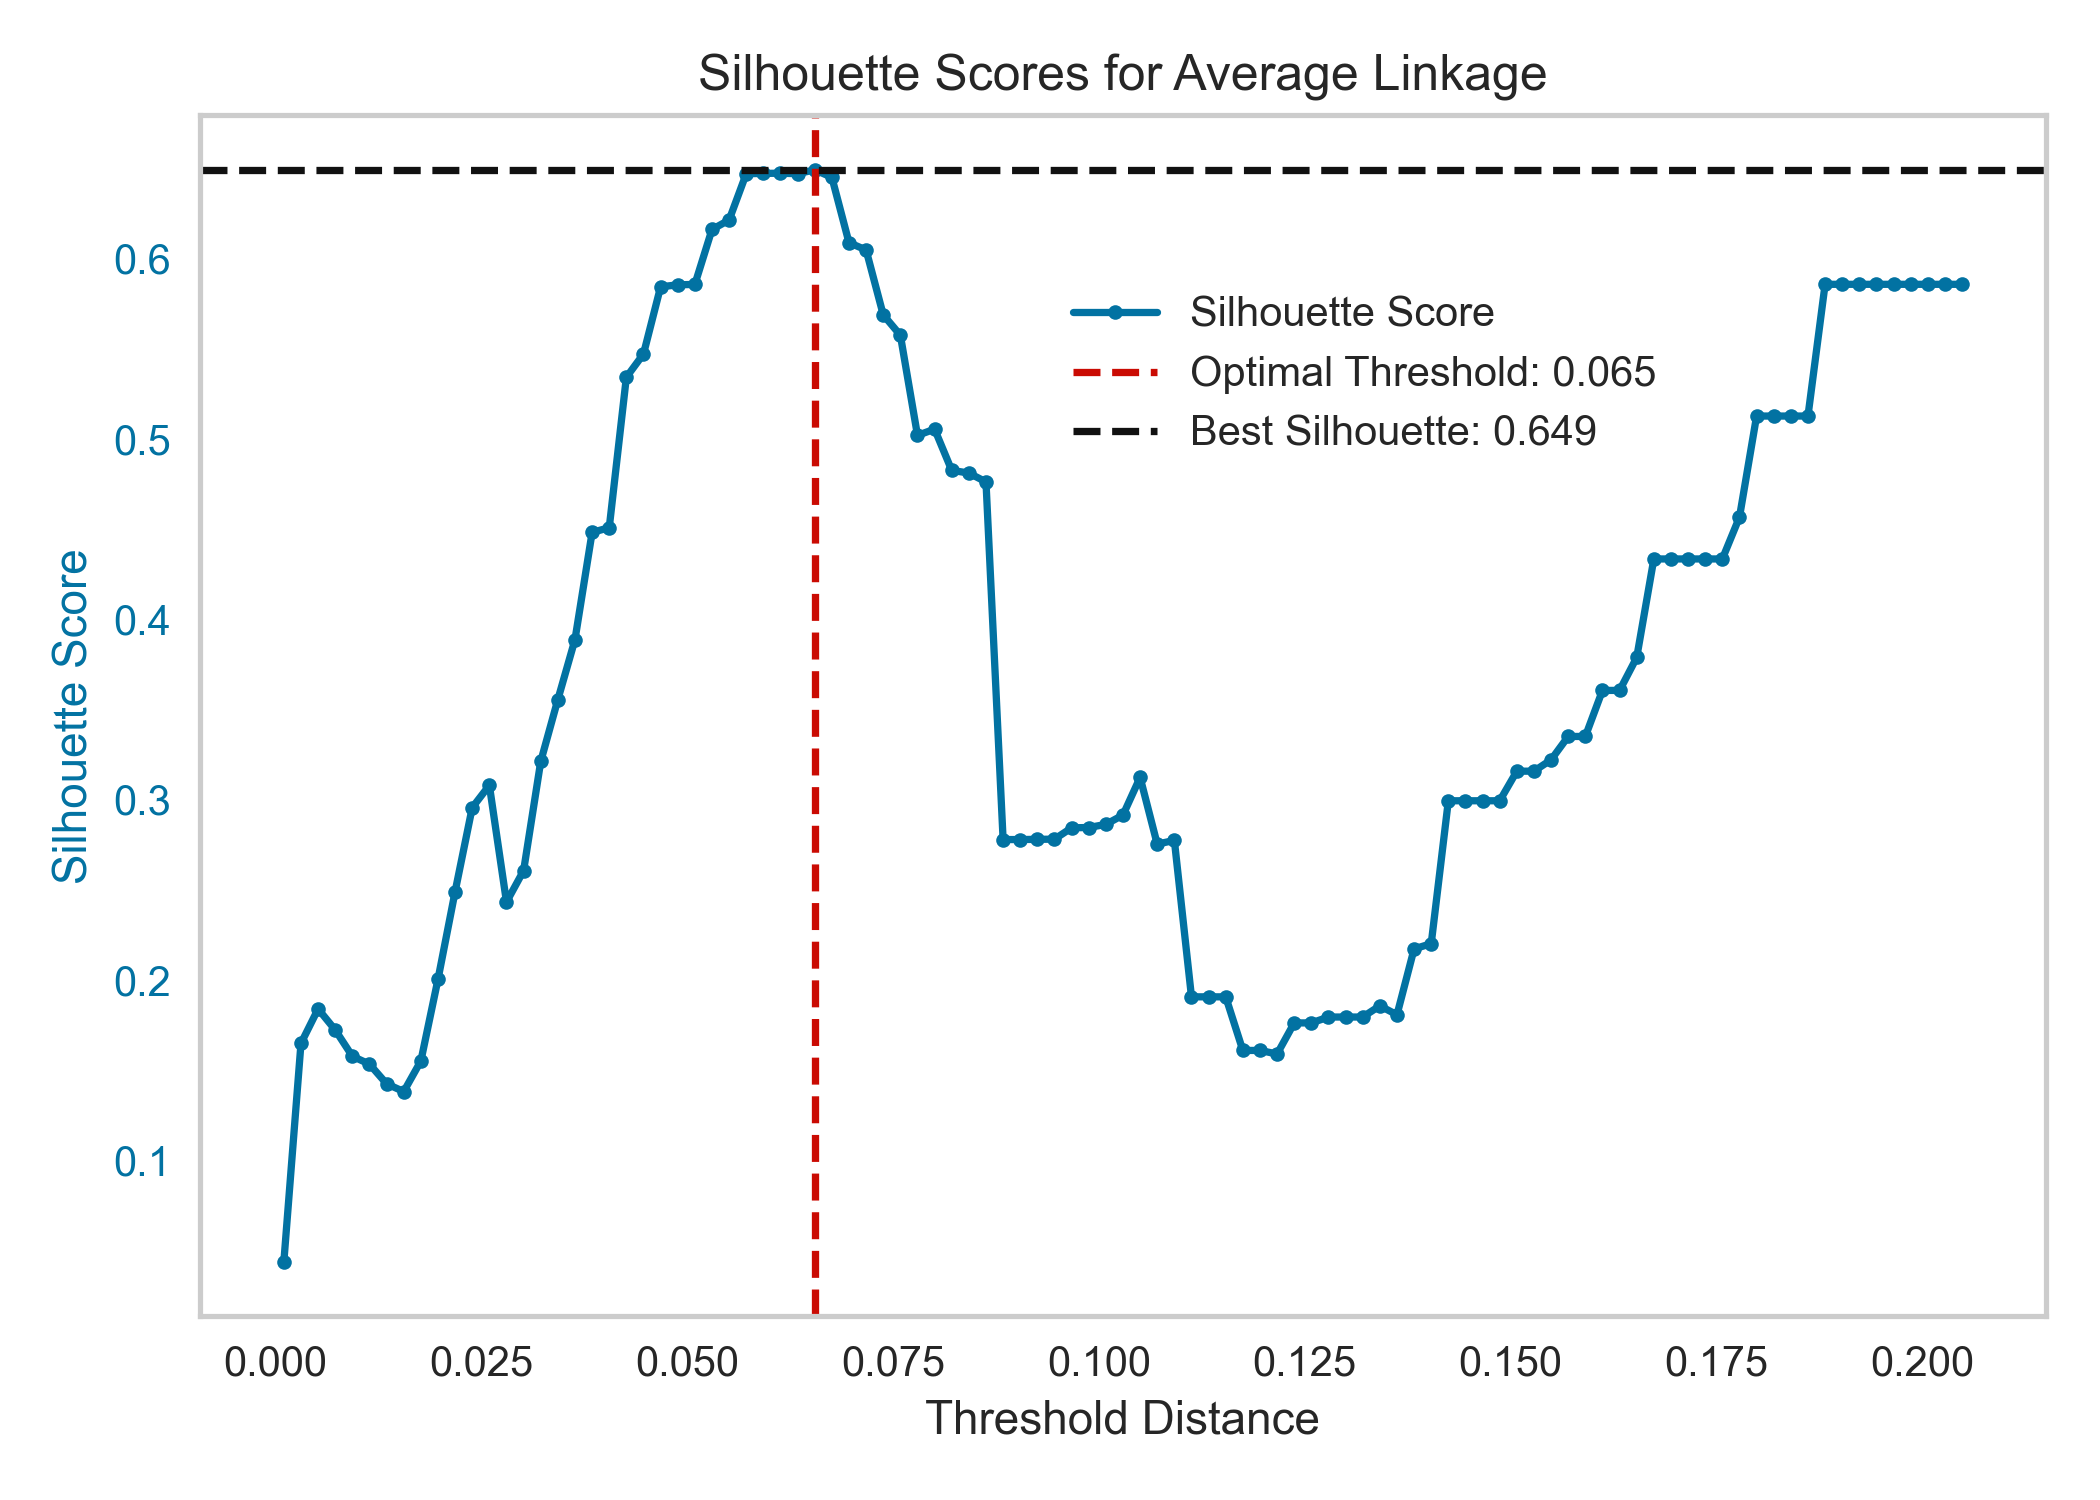
\includegraphics[width=0.45\textwidth]{images/silhouette_score_average_linkage.png}
    \caption{Silhouette score and number of anomalies with \textit{average} as linkage method at varying distance threshold. Optimal distance 0.065 with silhouette 0.649.}
    \label{fig:silhouette_score_average_linkage}
\end{figure}

\subsubsection{Determining the Optimal Threshold Distance}
To determine the optimal threshold distance, we selected the one with the highest Silhouette score. The Silhouette score measures how similar a data point is to its own cluster compared to other clusters. It is defined for each point \(i\) as:

\begin{equation}
    s(i) = \frac{b(i) - a(i)}{\max(a(i), b(i))}
\end{equation}

where:
\begin{itemize}
    \item \(a(i)\) is the average distance between \(i\) and all other points in the same cluster.
    \item \(b(i)\) is the minimum average distance between \(i\) and points in a different cluster.
\end{itemize}

The Silhouette score ranges from -1 to 1, where a higher score indicates better clustering performance, with points well matched to their own cluster and poorly matched to neighboring clusters. \newline
The Silhouette score was computed iteratively from 0.001 to the maximum height of the dendrogram, the distance where all points have been hierarchically clustered. The maximum height varies for different linkage methods due to the different ways they compute distances between clusters. \newline
The optimal threshold distance for average linkage corresponds to a distance of 0.065 with a Silhouette score of 0.649, while for complete linkage, the optimal threshold distance was 0.147 with a Silhouette score of 0.519.

\subsubsection{Identifying anomalies and probabilities}
\textbf{ONESTAMENTE TERREI SOLO IL METODO COMPLETE PERCHè RESTITUISCE MENO CLUSTER E MENO ANOMALIES (446 VS 561 A 20 CLUSTER RIMOSSI). PER SCREMARE UN PO'} \newline
To identify anomalies, clusters were sorted in descending sizes, and the cumulative sum of anomalies was computed by sequentially removing clusters. This process produced the curve of Figure [\ref{fig:anomalies_complete_linkage}].
The optimal number of clusters to remove was determined visually by choosing a threshold after which change to the number of anomalies became insignificant. We opted to remove the 20 largest clusters, leading to 446 anomalies. \newline
Next, we calculated the probability of each data point being an anomaly using an approach based on the 20th cluster as threshold. The increment in probability is computed as follows:

$$\begin{cases}
    \text{Before threshold:} & \Delta p = \frac{0.5}{\text{threshold}} \\
    \text{After threshold:} & \Delta p = \frac{0.5}{\text{total n. of clusters} - \text{threshold}}
\end{cases}$$

Each cluster was assigned a probability based on this approach, and each data point inherited the probability of its corresponding cluster. This method enabled a smooth transition in the anomaly probabilities.

\begin{figure}
    \centering
    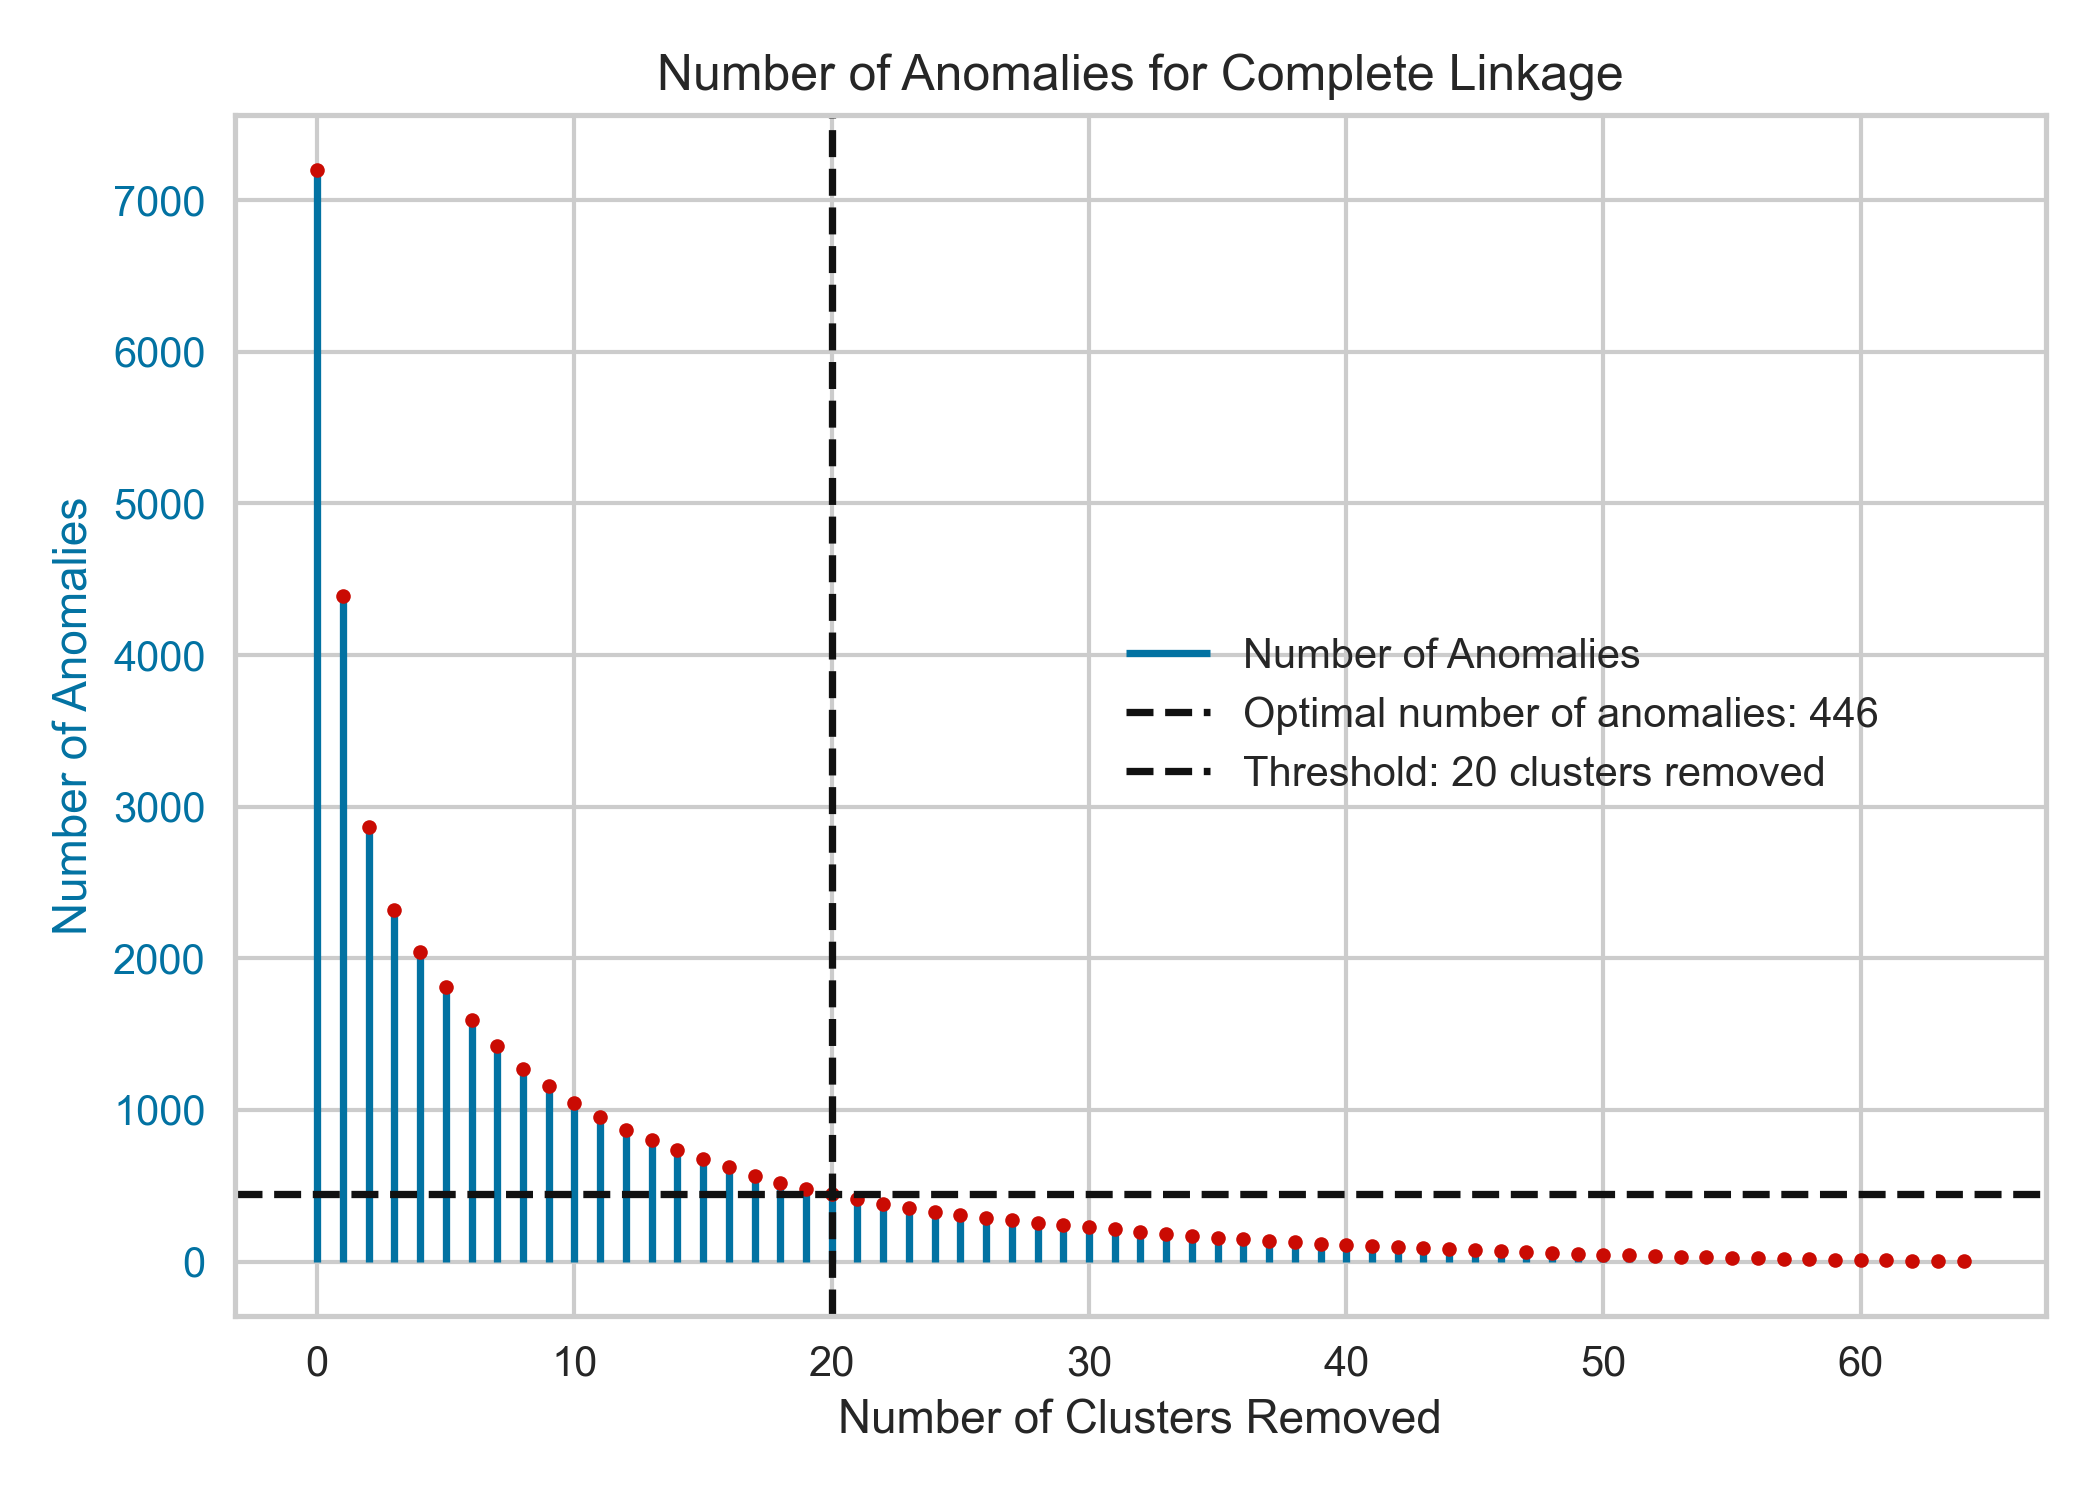
\includegraphics[width=0.45\textwidth]{images/anomalies_complete_linkage.png}
    \caption{Number of anomalies with \textit{complete} as linkage method at removal of clusters in decreasing order.}
    \label{fig:anomalies_complete_linkage}
\end{figure}

\begin{figure}
    \centering
    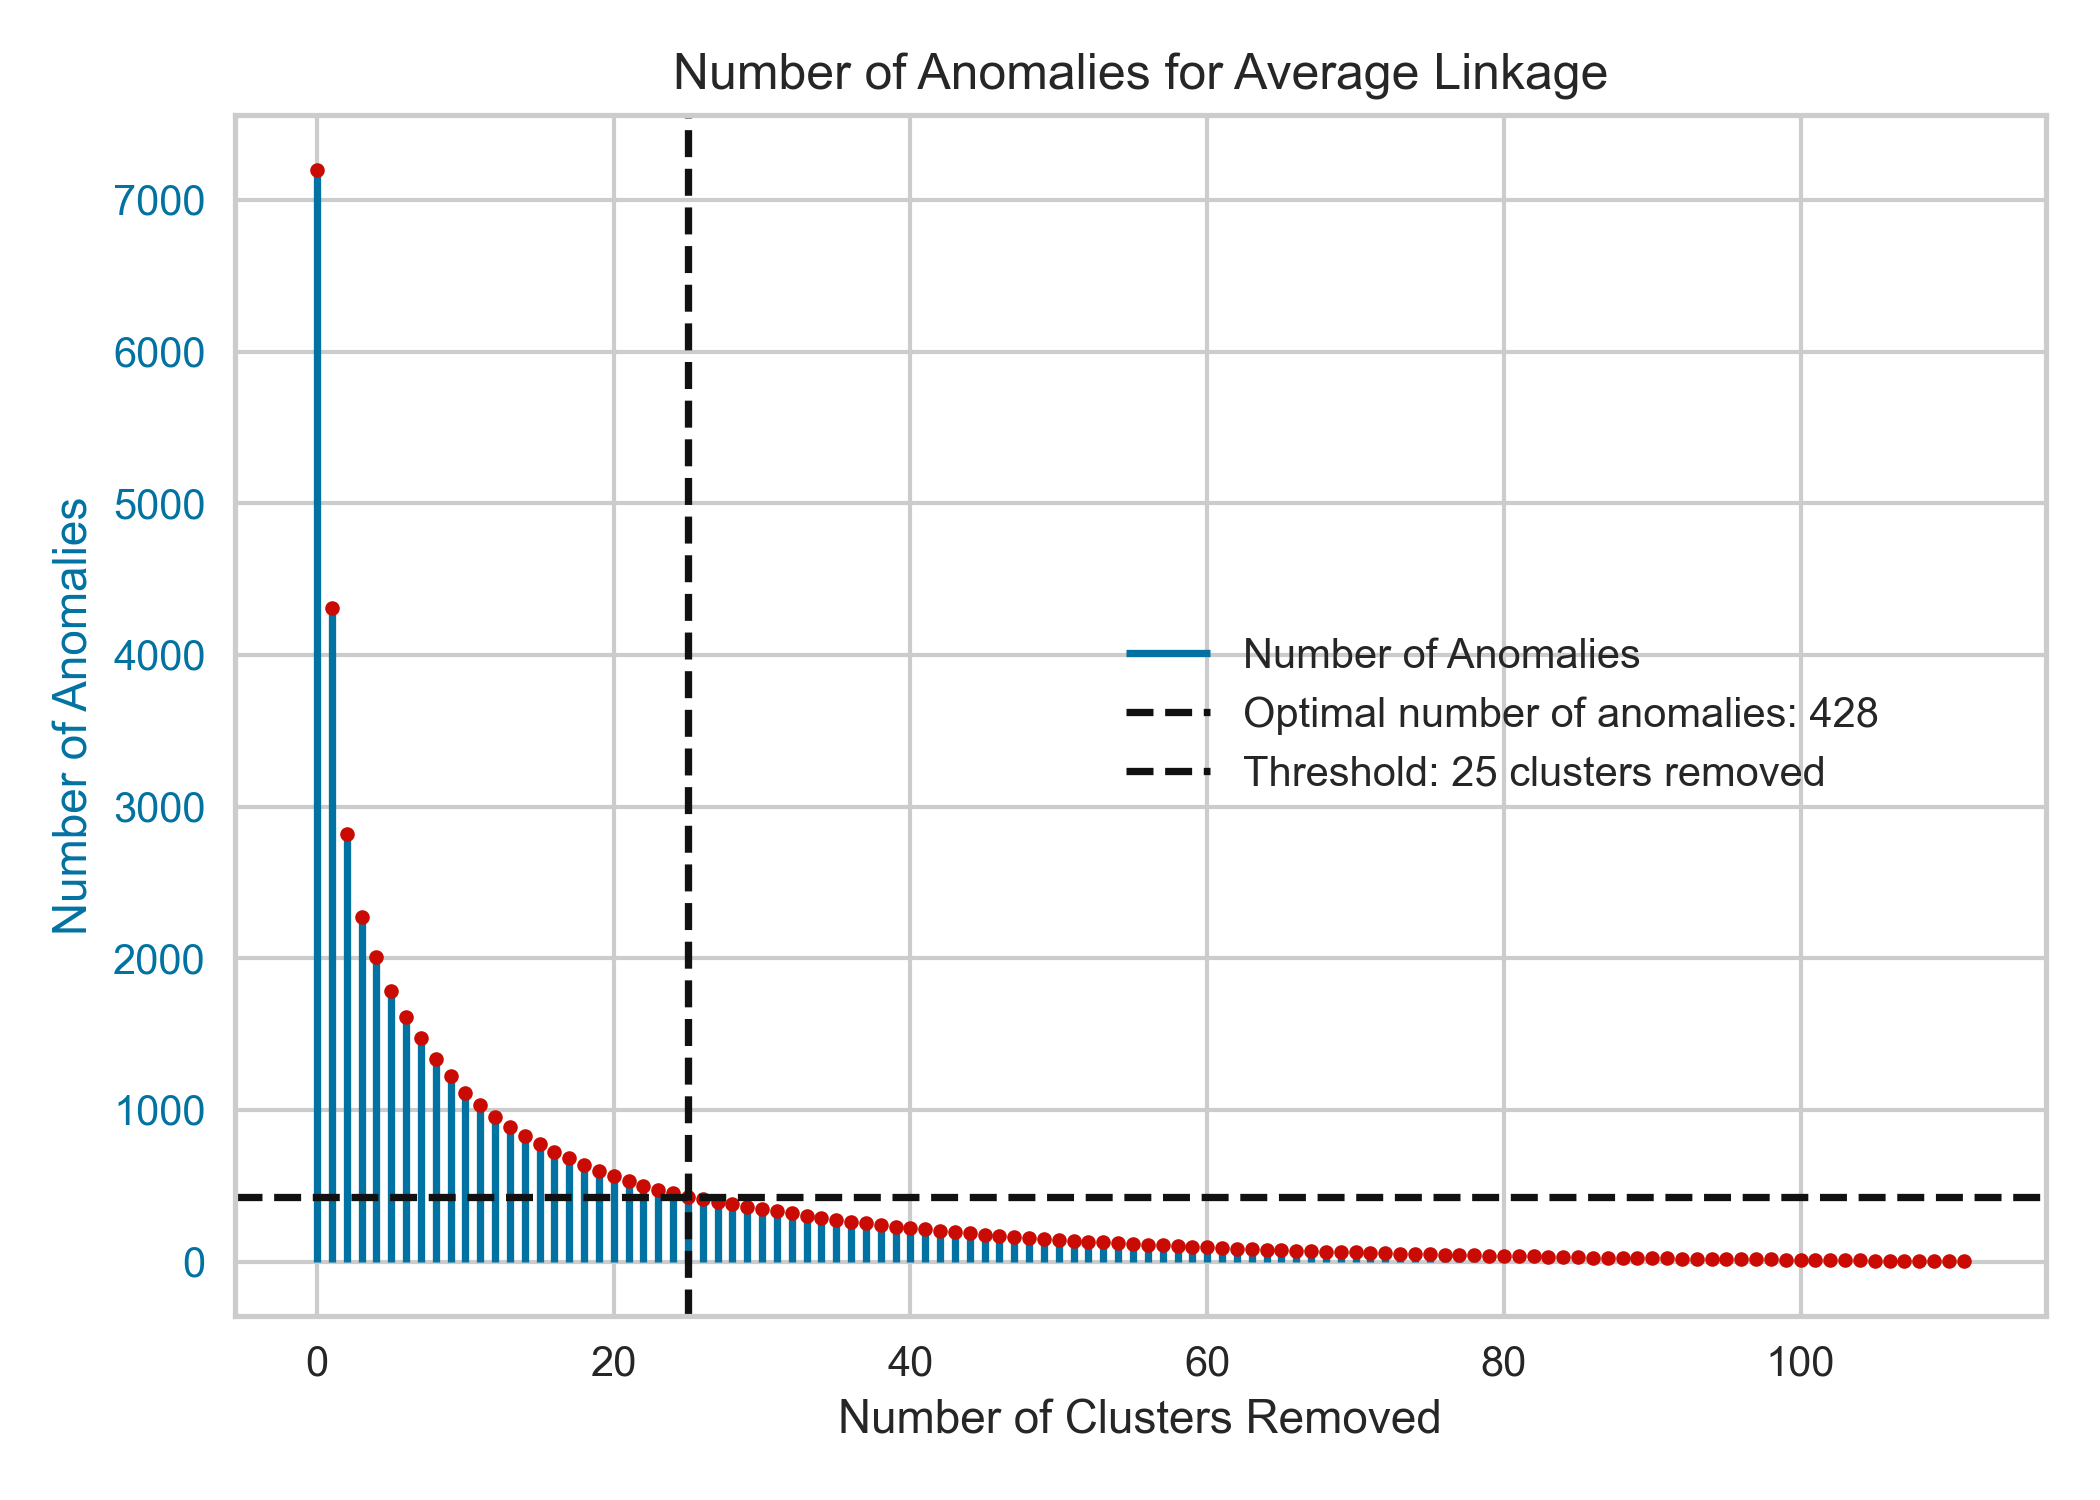
\includegraphics[width=0.45\textwidth]{images/anomalies_average_linkage.png}
    \caption{Number of anomalies with \textit{average} as linkage method at removal of clusters in decreasing order.}
    \label{fig:anomalies_average_linkage}
\end{figure}

The points identified as anomalies by the Linkage Methods are shown in Figure [\ref{fig:famd_hierarchical_average_fig}] and Figure [[\ref{fig:famd_hierarchical_complete_fig}]], plotted using FAMD for reducing the dimensionality from 21 features to 3 coordinates.

\begin{figure}
    \centering
    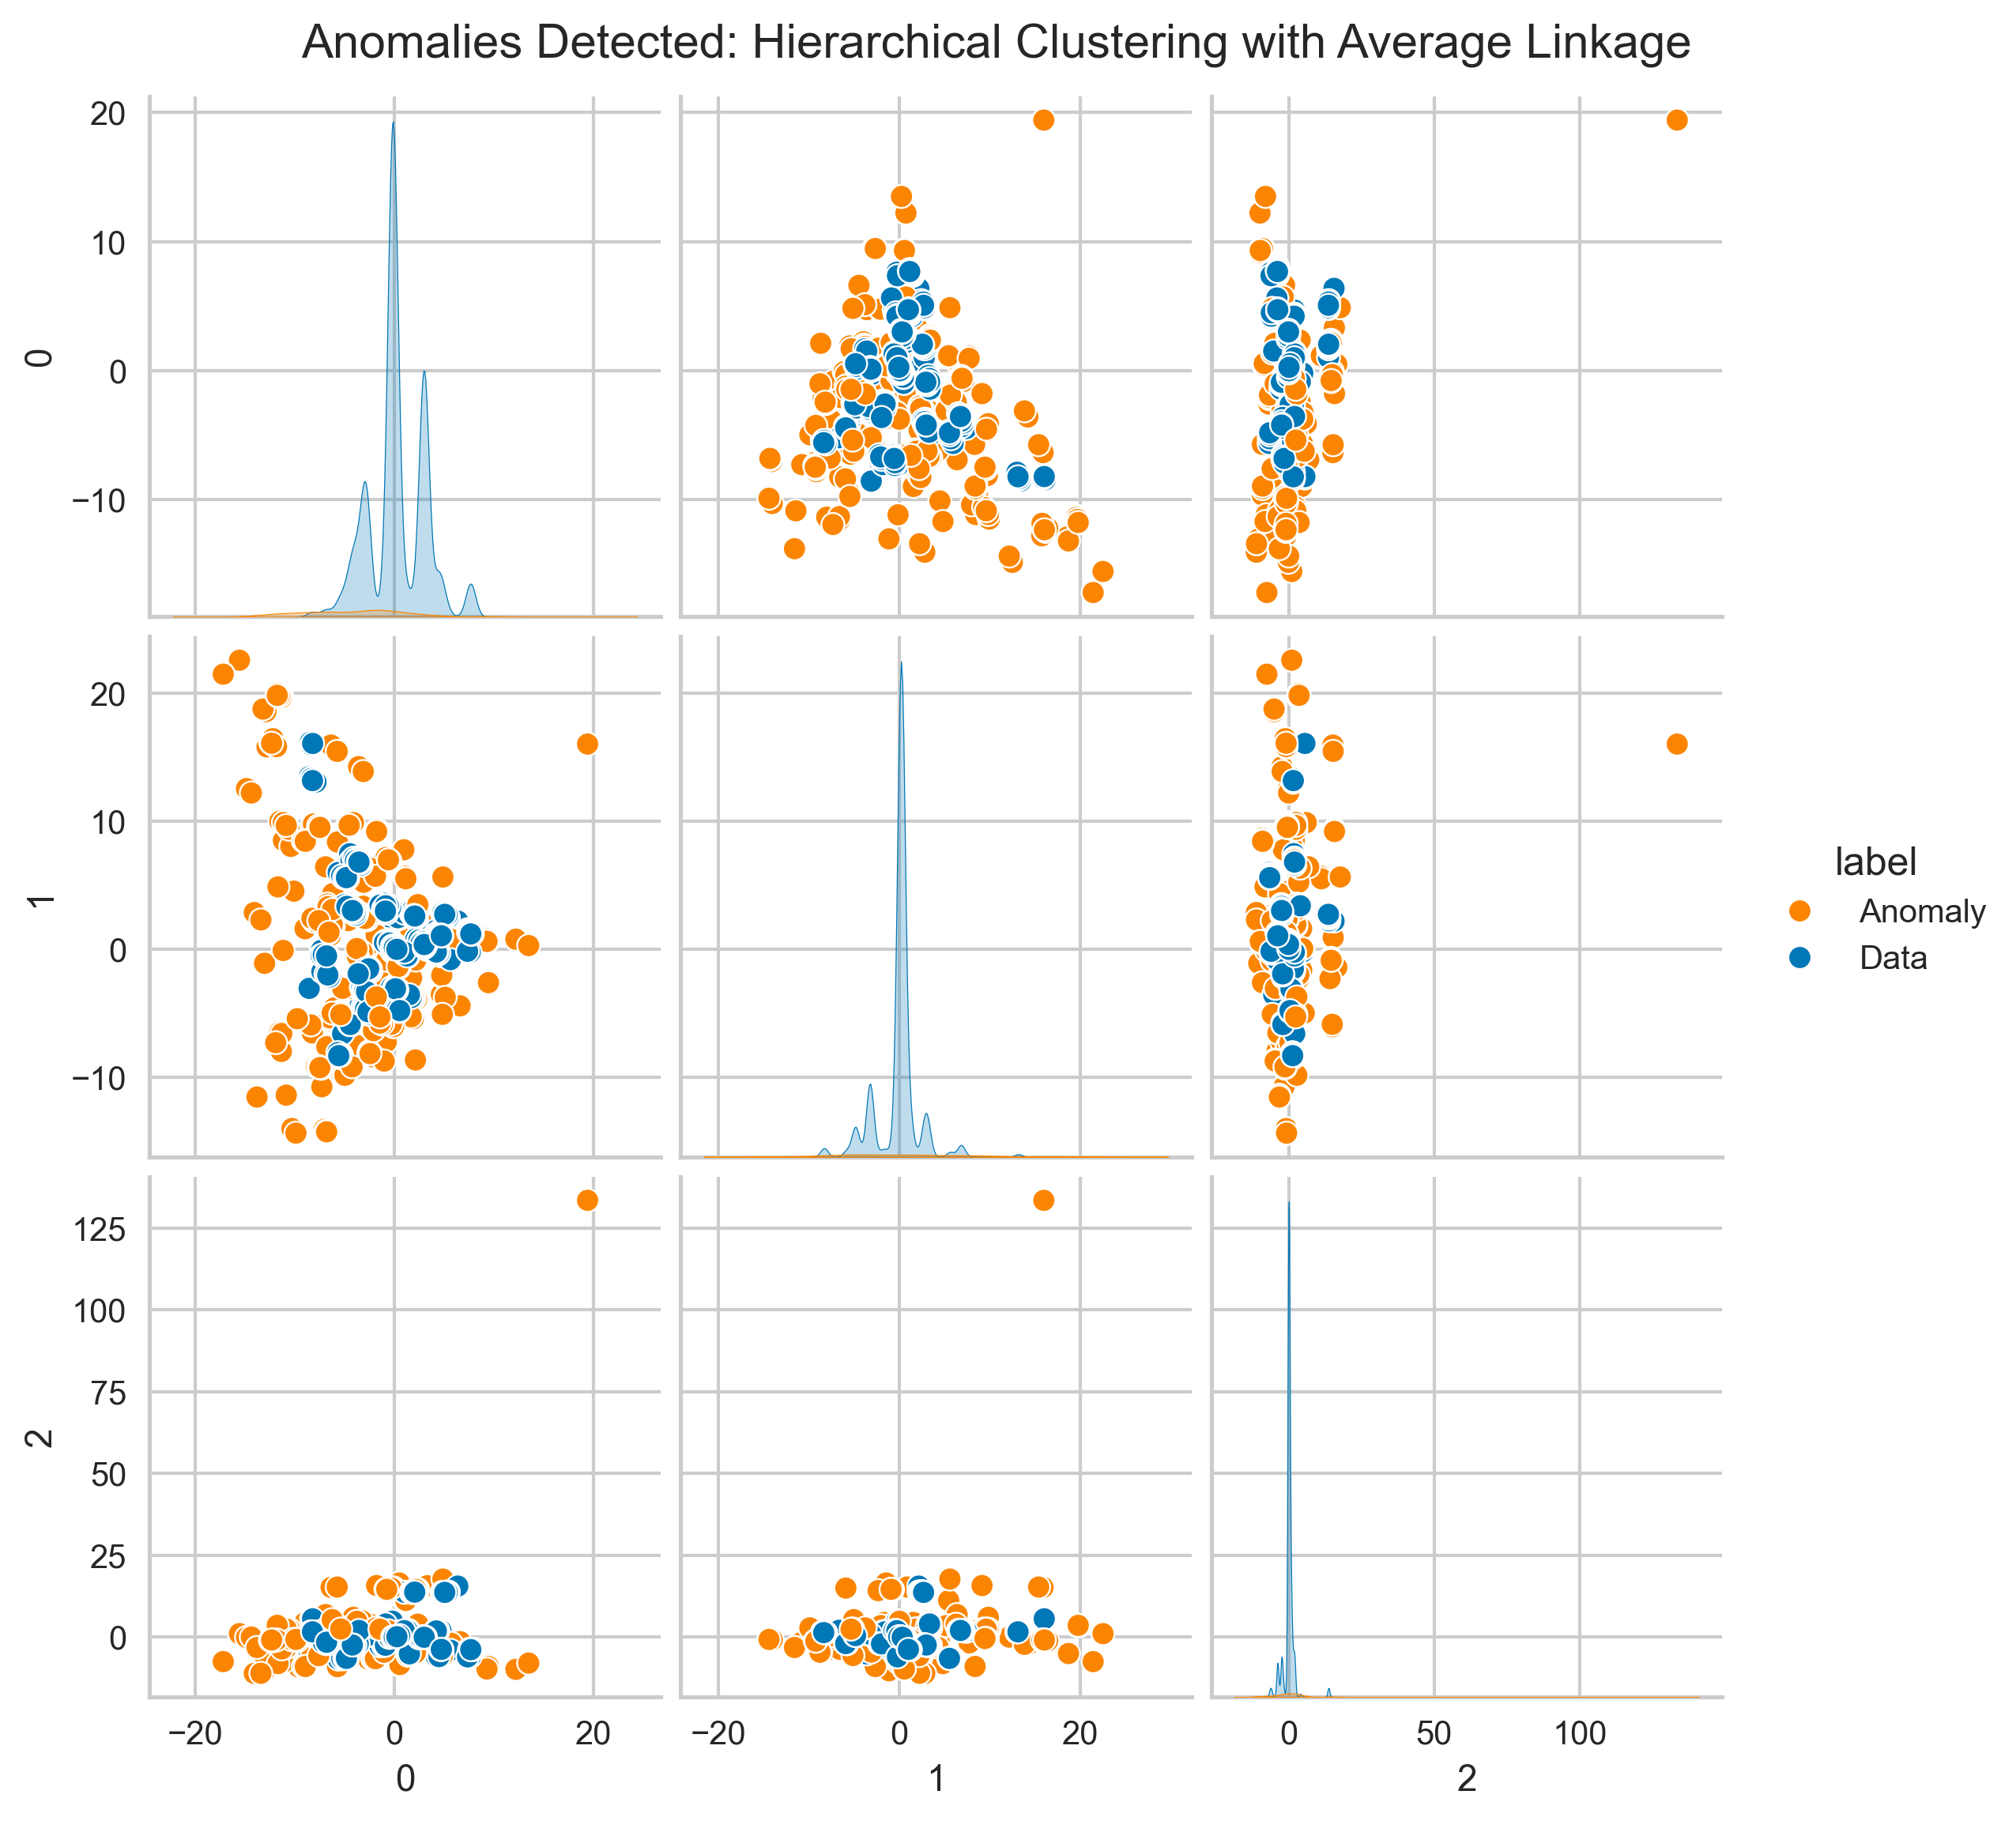
\includegraphics[width=0.45\textwidth]{images/famd_hierarchical_average_fig.png}
    \caption{Anomalies detected by Hierarchical Clustering with Average Linkage with $\epsilon$ \textbf{INSERIRE VALORI} outliers visualized on the 3 coordinates of FAMD.}
    \label{fig:famd_hierarchical_average_fig}
\end{figure}

\begin{figure}
    \centering
    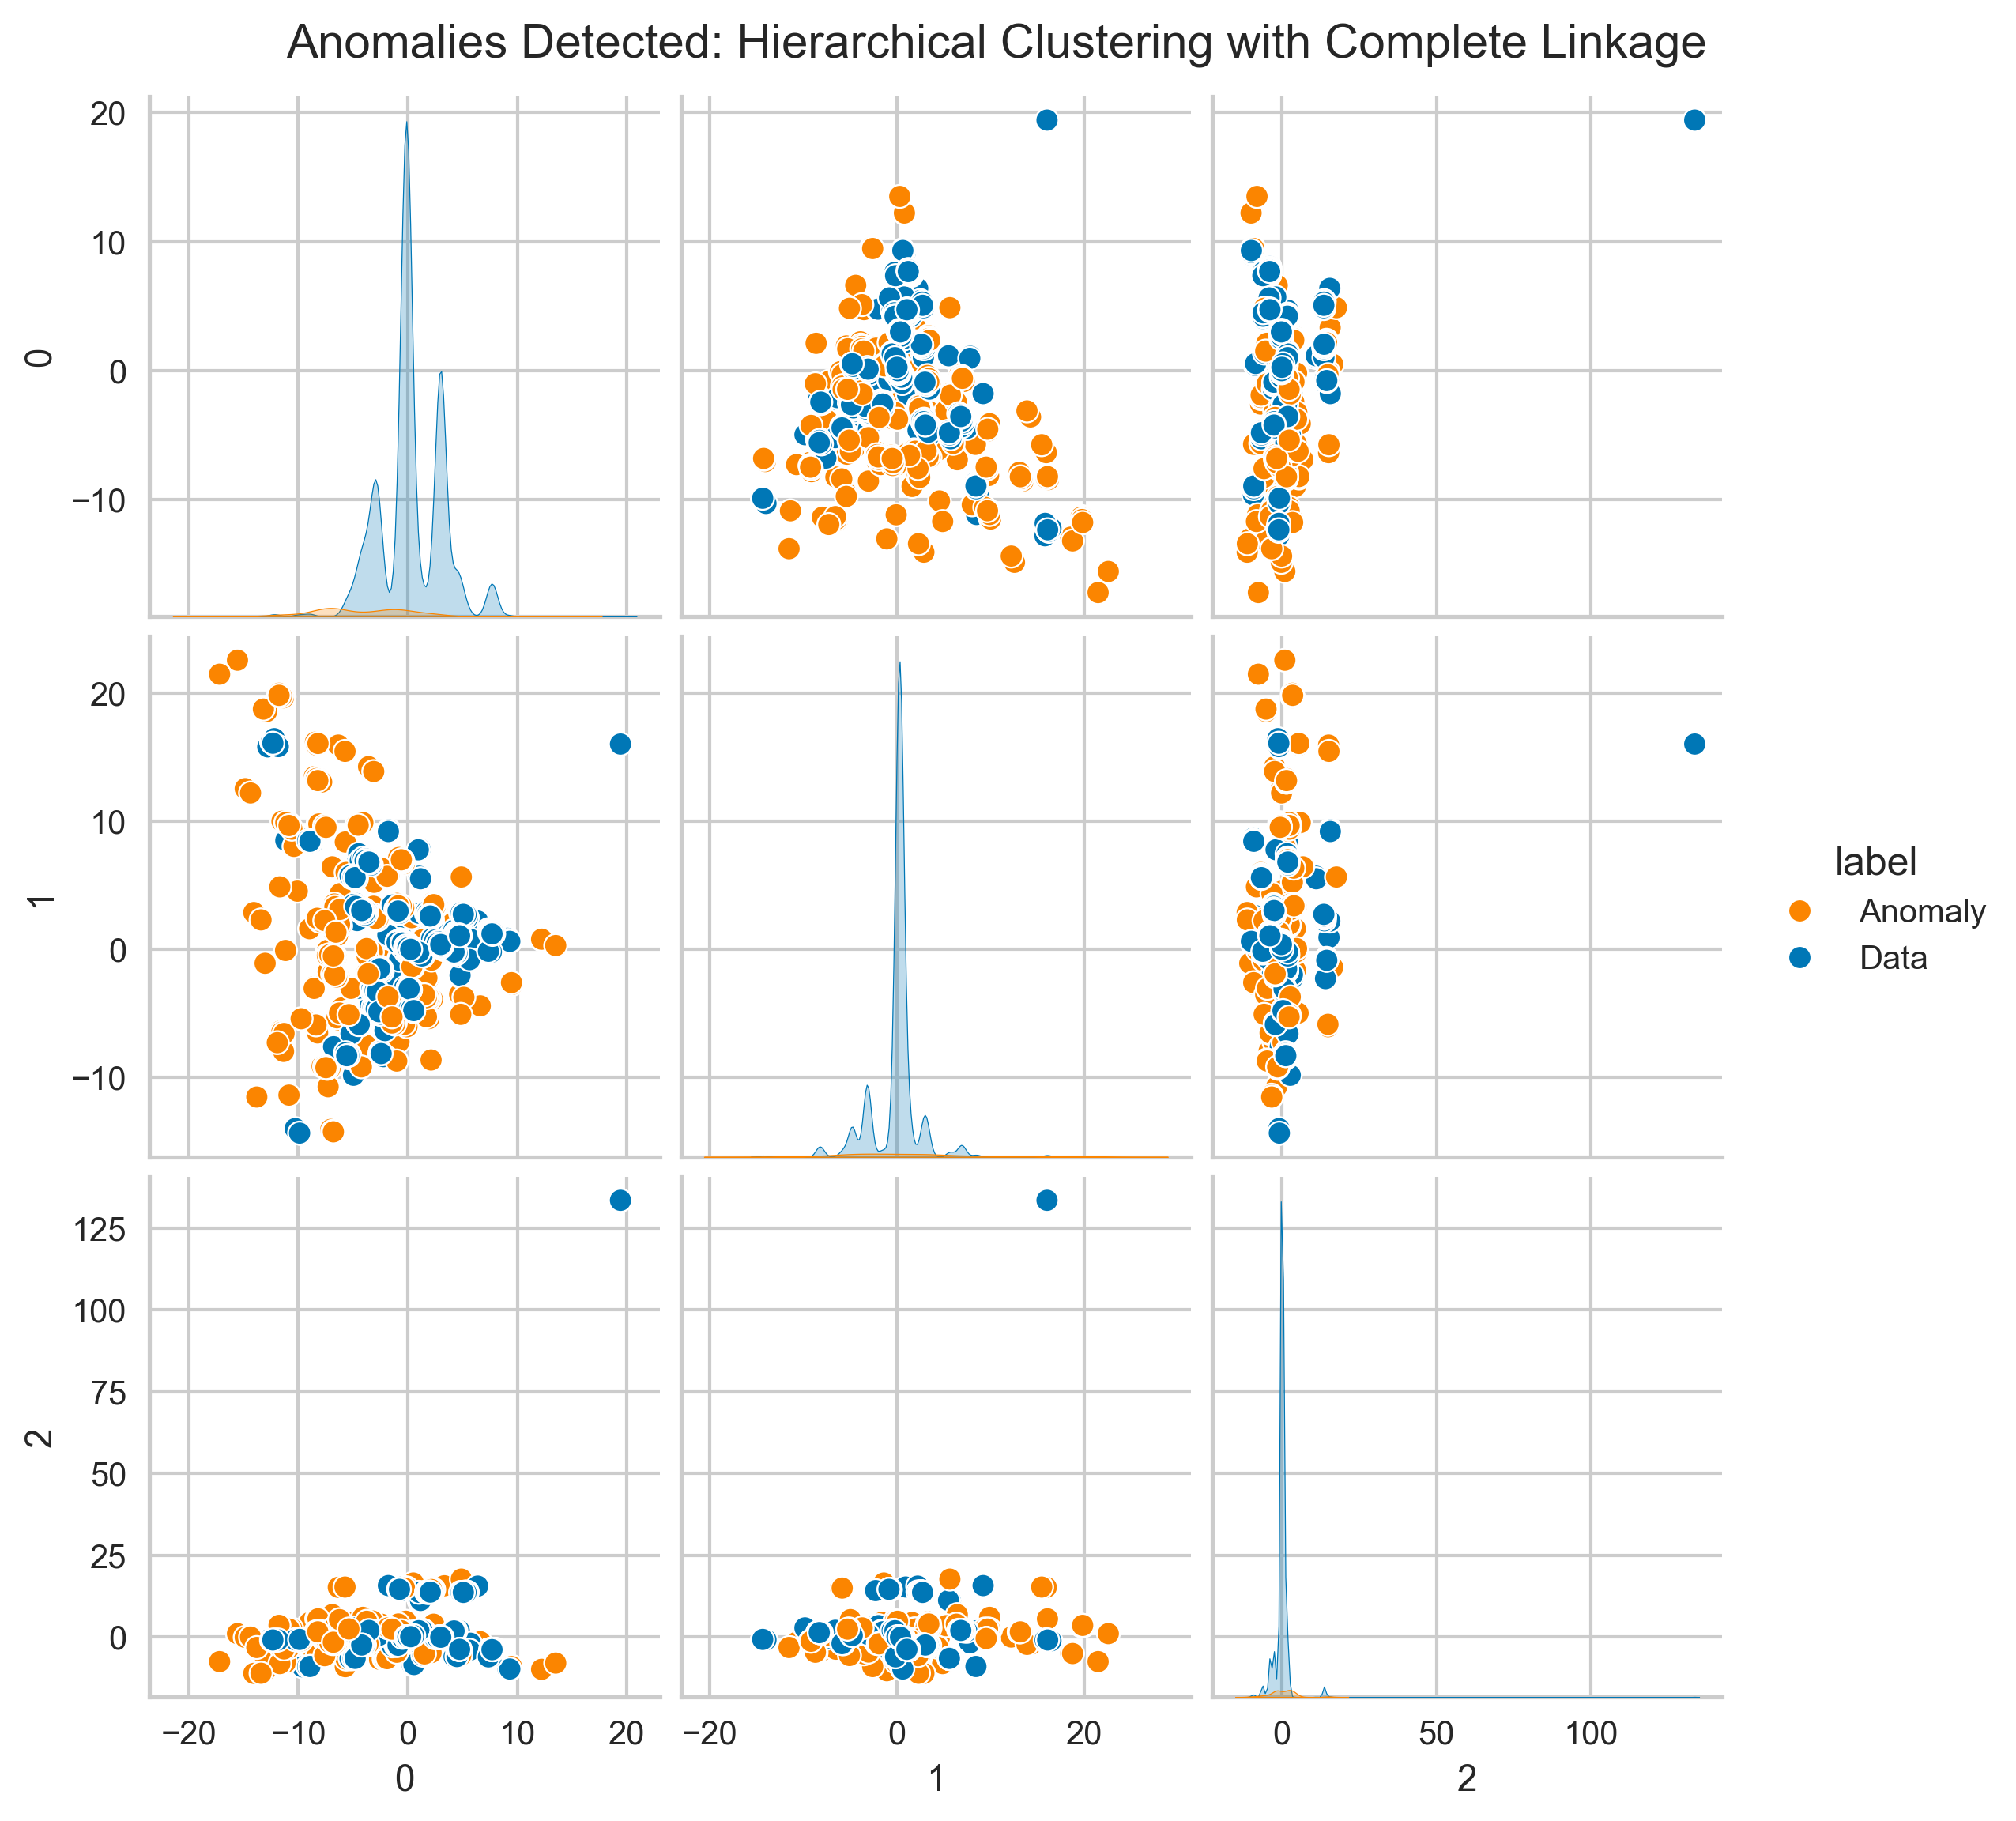
\includegraphics[width=0.45\textwidth]{images/famd_hierarchical_complete_fig.png}
    \caption{Anomalies detected by Hierarchical Clustering with Complete Linkage with $\epsilon$ \textbf{INSERIRE VALORI} outliers visualized on the 3 coordinates of FAMD.}
    \label{fig:famd_hierarchical_complete_fig}
\end{figure}

\subsection{K-Medoids}
K-Medoids is a variant of the popular K-Means clustering algorithm that is particularly well-suited for datasets containing mixed data types. Unlike K-Means, which uses the Euclidean distance to compute the mean of the cluster as its centroid, K-Medoids employs actual data points within the cluster as representatives, known as medoids. The medoid is defined as the data point that minimizes the sum of distances to all other points within the cluster. \newline
The advantage of K-Medoids over K-Means for datasets with mixed data types is that while K-means employs the Euclidean distance to compute the means, K-medoids can use a precomputed metric - the Gower distance in our case - to find the medoids, making it suitable for our dataset.
\subsubsection{Determining the optimal number of clusters}
To determine the optimal number of clusters for the dataset, we employed the elbow method. This method identifies the point at which adding more clusters does not significantly improve the clustering performance, balancing model complexity and performance. The elbow method was necessary because hierarchical clustering with Ward's method, which is suitable for producing compact and spherical clusters, requires the use of Euclidean distance, which is not ideal for our mixed-type dataset. \newline
The elbow for the case of K-Medoids is shown in Figure \ref{fig:elbowkmedoids}, indicating an optimal number of clusters equal to five. After determining the optimal number of clusters and fitting the data, K-Medoids returns the indices of the elements corresponding to the medoids of the clusters. \newline
\subsubsection{Identifying Anomalies}
Anomalies were identified by assessing the distance of each element from its nearest medoid: the closer an observation is to its nearest medoid, the lower the probability that the observation is an anomaly. Elements deviating by more than a specified number of standard deviations from the mean distance within the same cluster were considered anomalies. Figure \ref{fig:kmedoidsAnomalies} illustrates the number of anomalies identified for each threshold. We opted to adopt a threshold value of 4.3, correlating to a count of 343 anomalies denoted by a red dotted line. This specific threshold was selected because beyond this value, the reduction in the number of anomalies detected exhibits a less pronounced decline, affecting fewer elements. Since anomalies are considered deviations from the norm, our objective is to identify a point beyond which further increases in the threshold value yield minimal changes in the count of anomalies detected. The selected threshold denotes the point at which the probability of an element being an anomaly exceeds 0.5. Consequently, rounding the probability for each element precisely mirrors the partitioning of the dataset established using the chosen threshold.
The points identified as anomalies by K-Medoids are shown in Figure [\ref{fig:famd_kmedoids}], plotted using FAMD for reducing the dimensionality from 21 features to 3 coordinates.


\begin{figure}
    \centering
    \includegraphics[width=0.45\textwidth]{images/ElbowKMedoids.png}
    \caption{Elbow visualization for K-Medoids}
    \label{fig:elbowkmedoids}
\end{figure}


\begin{figure}
    \centering
    \includegraphics[width=0.45\textwidth]{images/KMedoidsAnomalies.png}
    \caption{Number of anomalies for each threshold value for K-Medoids. The dotted line represent a threshold value of 4.3 standard deviations, corresponding to 343 anomalies}
    \label{fig:kmedoidsAnomalies}
\end{figure}

\begin{figure}
    \centering
    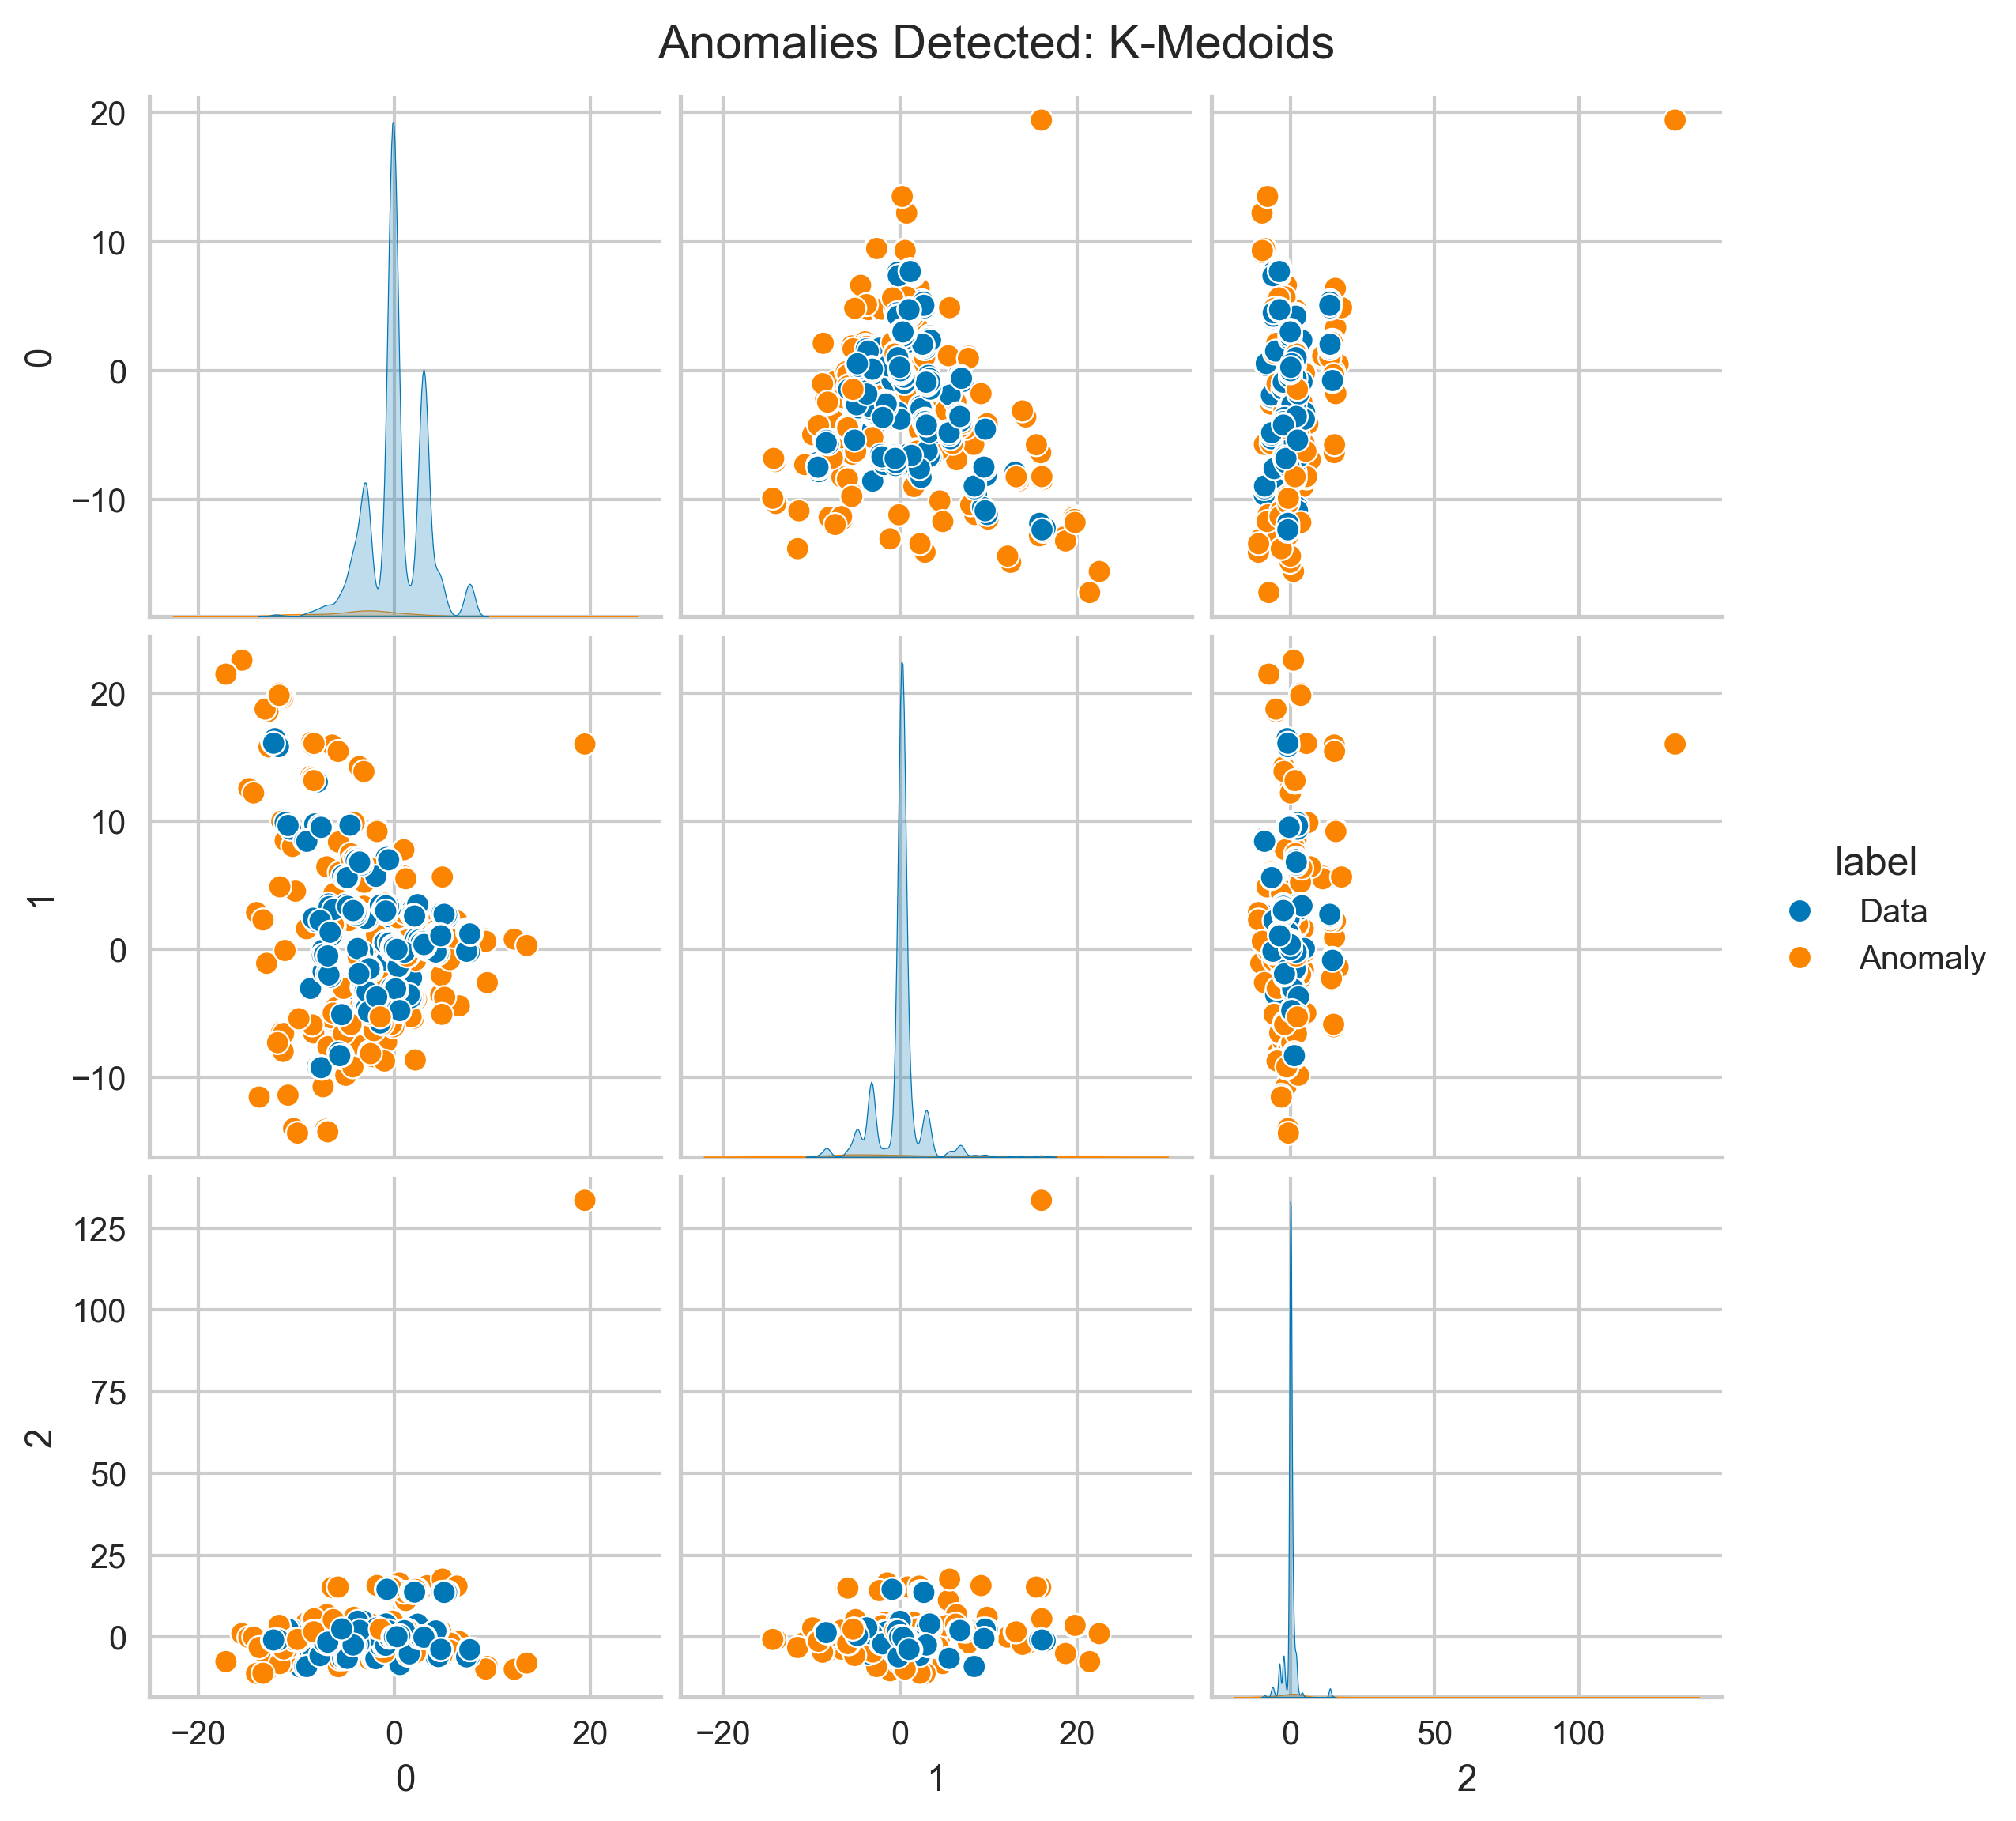
\includegraphics[width=0.45\textwidth]{images/famd_kmedoids.png}
    \caption{Anomalies detected by K-Medoids with $\epsilon$ \textbf{INSERIRE VALORI} outliers visualized on the 3 coordinates of FAMD.}
    \label{fig:famd_kmedoids}
\end{figure}

\subsection{K-prototypes}
Similarly with K-Medoids, we also employed the use of K-Prototype, which can also handle mixed data types but unlike K-Medoids, it uses prototypes, which are synthetic points representing the cluster. For numerical attributes, the prototype is the mean of the cluster. For categorical attributes, the prototype is the mode (most frequent category) of the cluster. Moreover, while in the case of K-Medoids, the medoid is an actual data point from the dataset that is part of the cluster, in K-Prototype the prototype is a synthetic point and does not necessarily correspond to an actual data point in the dataset.

\section{Density Based Clustering}
Density-based clustering is a powerful technique for identifying clusters of arbitrary shape and separating noise or anomalies from the underlying clusters. Unlike distance-based methods like K-Means or K-Medoids, density-based clustering algorithms do not require a predefined number of clusters. Instead, they group data points based on their local density, considering both the density of the points themselves and their spatial proximity.
One of the most widely used density-based clustering algorithms is DBSCAN (Density-Based Spatial Clustering of Applications with Noise), which was introduced by Sander et al. in 1998 \cite{Sander-etal98}. DBSCAN is particularly effective in handling datasets with noise and anomalies, as it can identify and separate these points from the main clusters.

\subsection{DBSCAN}
DBSCAN (Density-Based Spatial Clustering of Applications with Noise) is a density-based clustering algorithm that groups data points based on two key parameters: \textit{epsilon} ($\epsilon$) and \textit{minimum points} (\textit{minPts}). The algorithm operates by calculating the number of points within a radius $\epsilon$ around each point $p$. If the number of points is greater than or equal to minPts, $p$ is classified as a core point. Points within the $\epsilon$-neighborhood of a core point are assigned to the same cluster, and core points are connected if they are density-reachable. Border points, which lie within the $\epsilon$-neighborhood of a core point but are not core points themselves, are also assigned to the clusters. Points that are neither core nor border points are considered noise or anomalies. \newline
The main advantages of DBSCAN are that it can identify clusters of arbitrary shape and size and is robust to noise and anomalies. However, this technique is sensitive to varying densities and cluster sizes.
\subsubsection{Determining the Optimal $\epsilon$ and \textit{minPts}}
Choosing the appropriate parameters $\epsilon$ and \textit{minPts} for DBSCAN is crucial for obtaining good clustering results. A common heuristic for determining \textit{minPts} is to set it to twice the number of features in the dataset, as suggested by Sander et al. \cite{Sander-etal98}. In our case, with 21 features, \textit{minPts} was set to 42. \newline
To find a suitable starting value for the $\epsilon$ parameter, we computed the distance of each point to its $k^{th}$ nearest neighbor, ordered these distances, and plotted them as shown in Figure [\ref{fig:dbscan_epsilon_knee}]. 

\begin{figure}
    \centering
    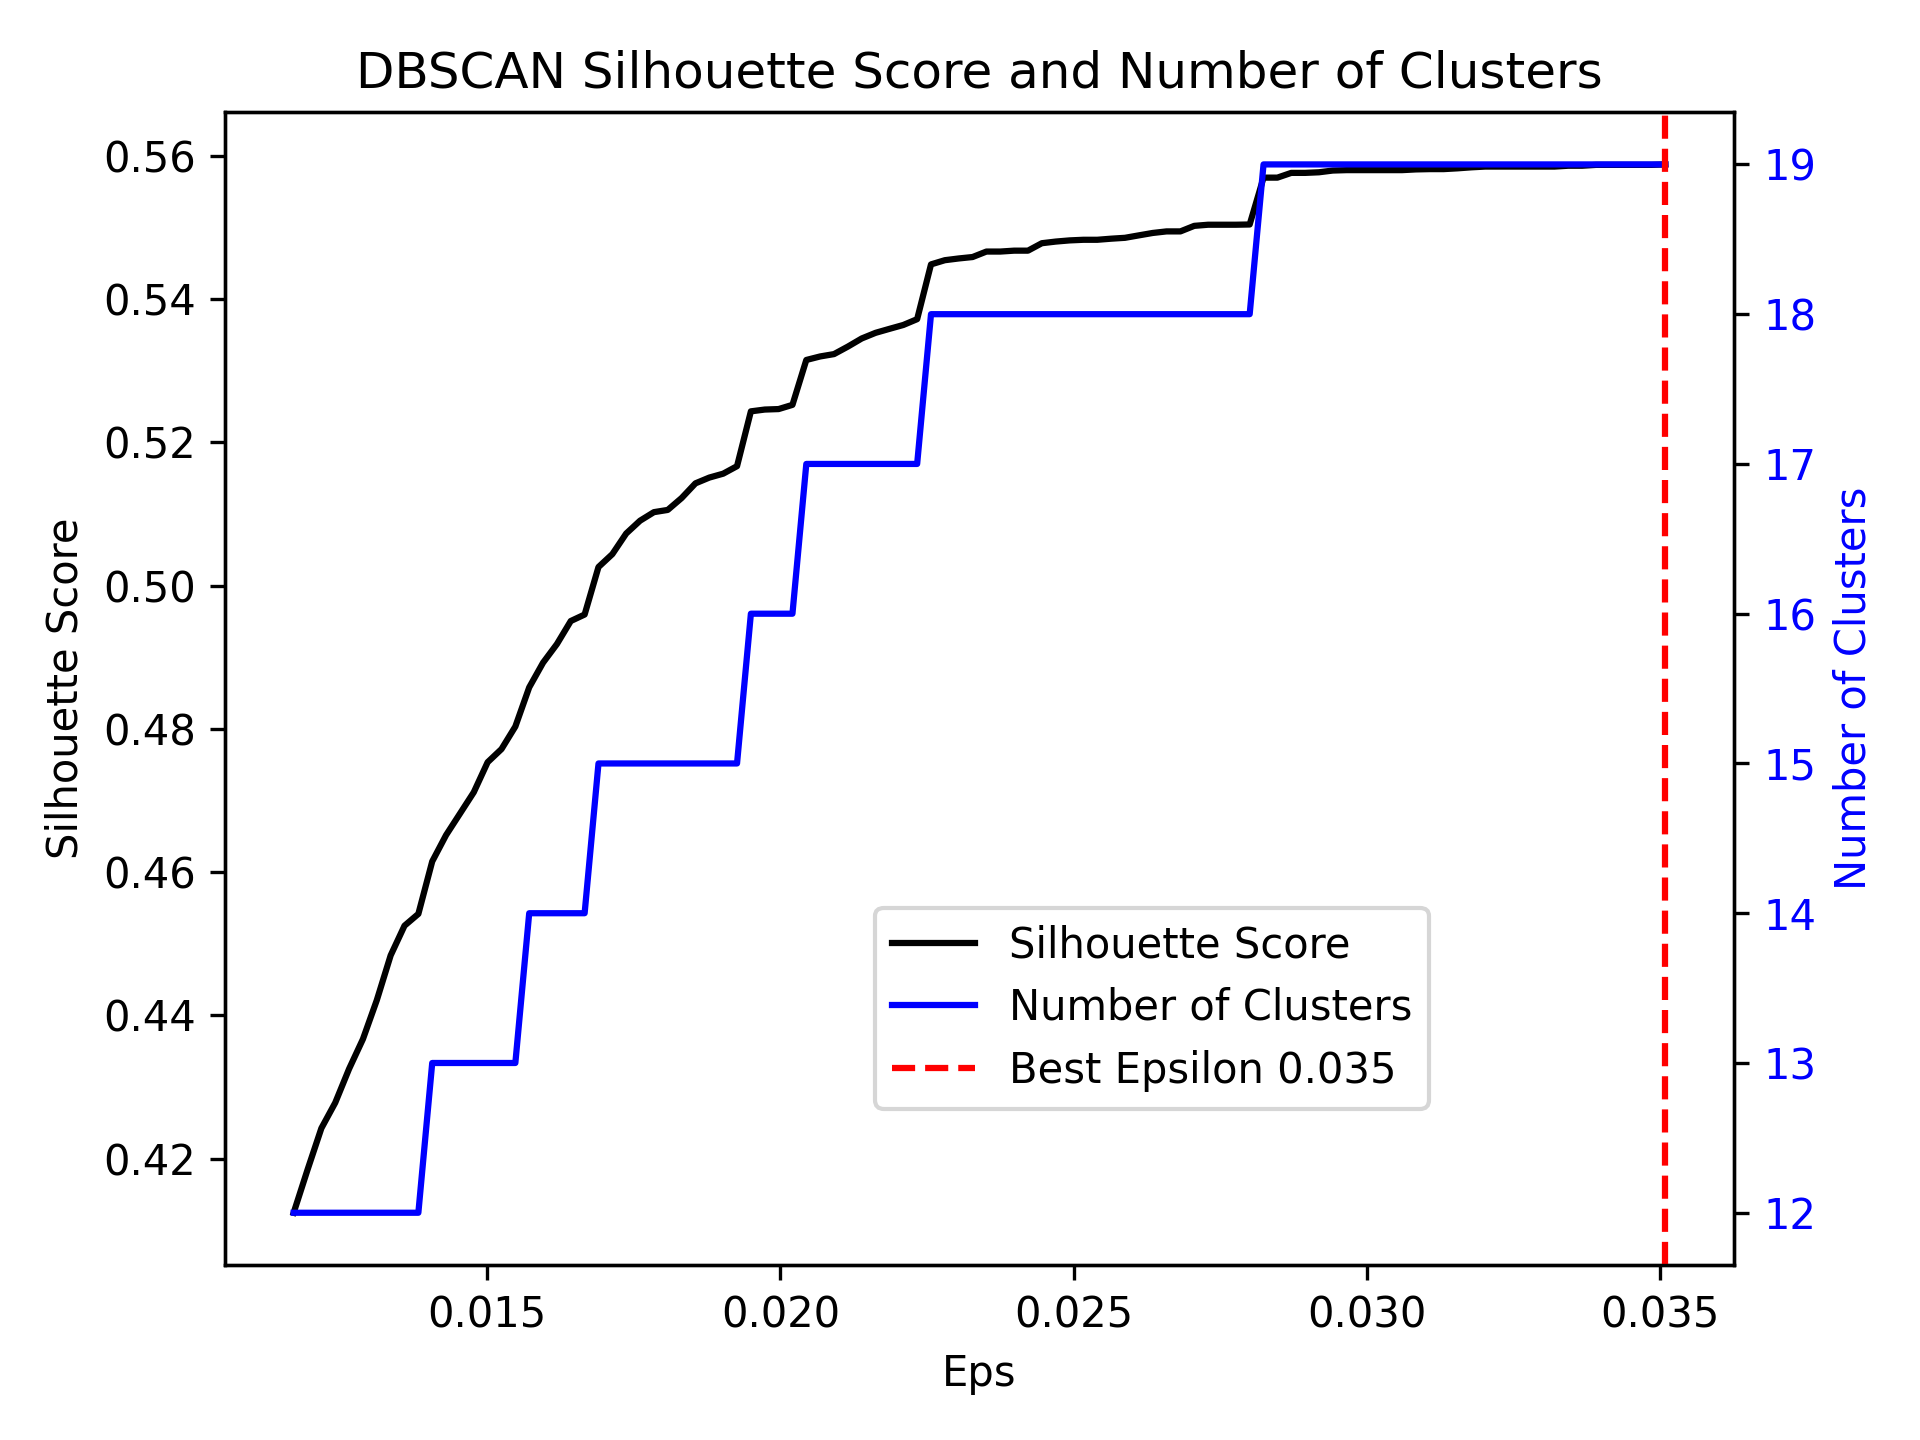
\includegraphics[width=0.45\textwidth]{images/dbscan_silhouette.png}
    \caption{DBSCAN Silhouette Score and Number of Cluster at the variation of $\epsilon$}
    \label{fig:dbscan_silhouette}
\end{figure}

The knee of this curve was identified as an initial estimate for $\epsilon$. We then performed DBSCAN iteratively within the range $$[0.5 \times \text{initial estimate}, 1.5 \times \text{initial estimate}]$$ and selected the $\epsilon$ value that yielded the highest Silhouette score. The results of this process are illustrated in Figure [\ref{fig:dbscan_silhouette}]. The Silhouette score stabilized after 0.030, and the best $\epsilon$ value was found to be 0.035.

\begin{figure}
    \centering
    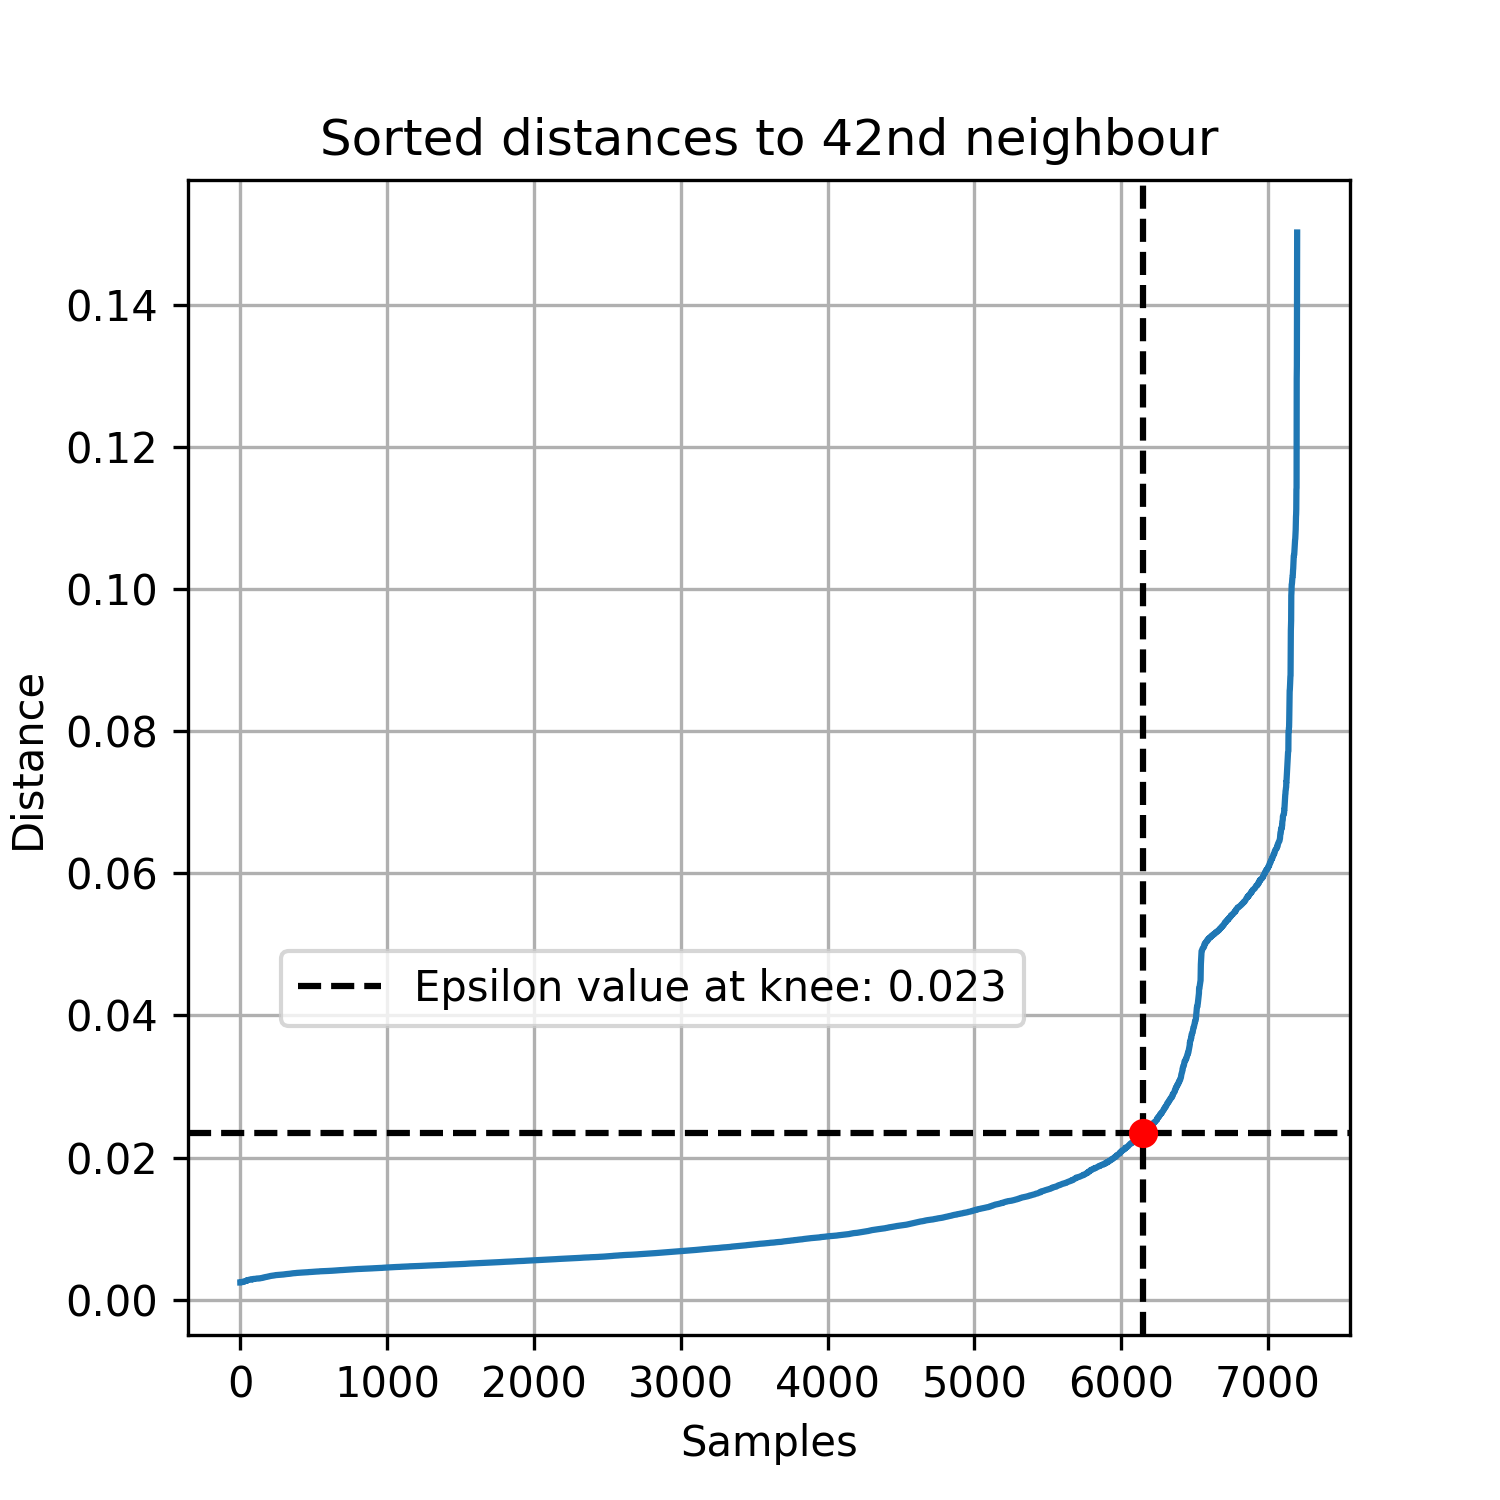
\includegraphics[width=0.45\textwidth]{images/dbscan_epsilon_knee.png}
    \caption{Sorted distances to $42^{nd}$ neighbour}
    \label{fig:dbscan_epsilon_knee}
\end{figure}

\subsubsection{Identifying Anomalies}
\textbf{CORREGGERE IL METODO DI CALCOLO PROBABILITà}

To compute the probability of each point being an anomaly using DBSCAN, we followed a systematic approach. For each point, we calculated the density, defined as the number of points within the radius $\epsilon$. The points classified by DBSCAN as noise (labelled as -1 by the algorithm) were assigned a probability of 1, indicating they are definite anomalies. Core points, with densities greater than or equal to \textit{minPts}, were assigned a probability of 0, indicating they are not anomalies. \newline
For other points, the anomaly probability was inversely proportional to their density. Specifically, the density values were normalized to the range [0, 1], and the anomaly probability was set as $1 - \text{normalized density}$. This ensures that points with higher densities have lower anomaly probabilities, while points with lower densities have higher probabilities.
The points identified as anomalies by DBSCAN are shown in Figure [\ref{fig:famd_dbscan}], plotted using FAMD for reducing the dimensionality from 21 features to 3 coordinates.

\begin{figure}
    \centering
    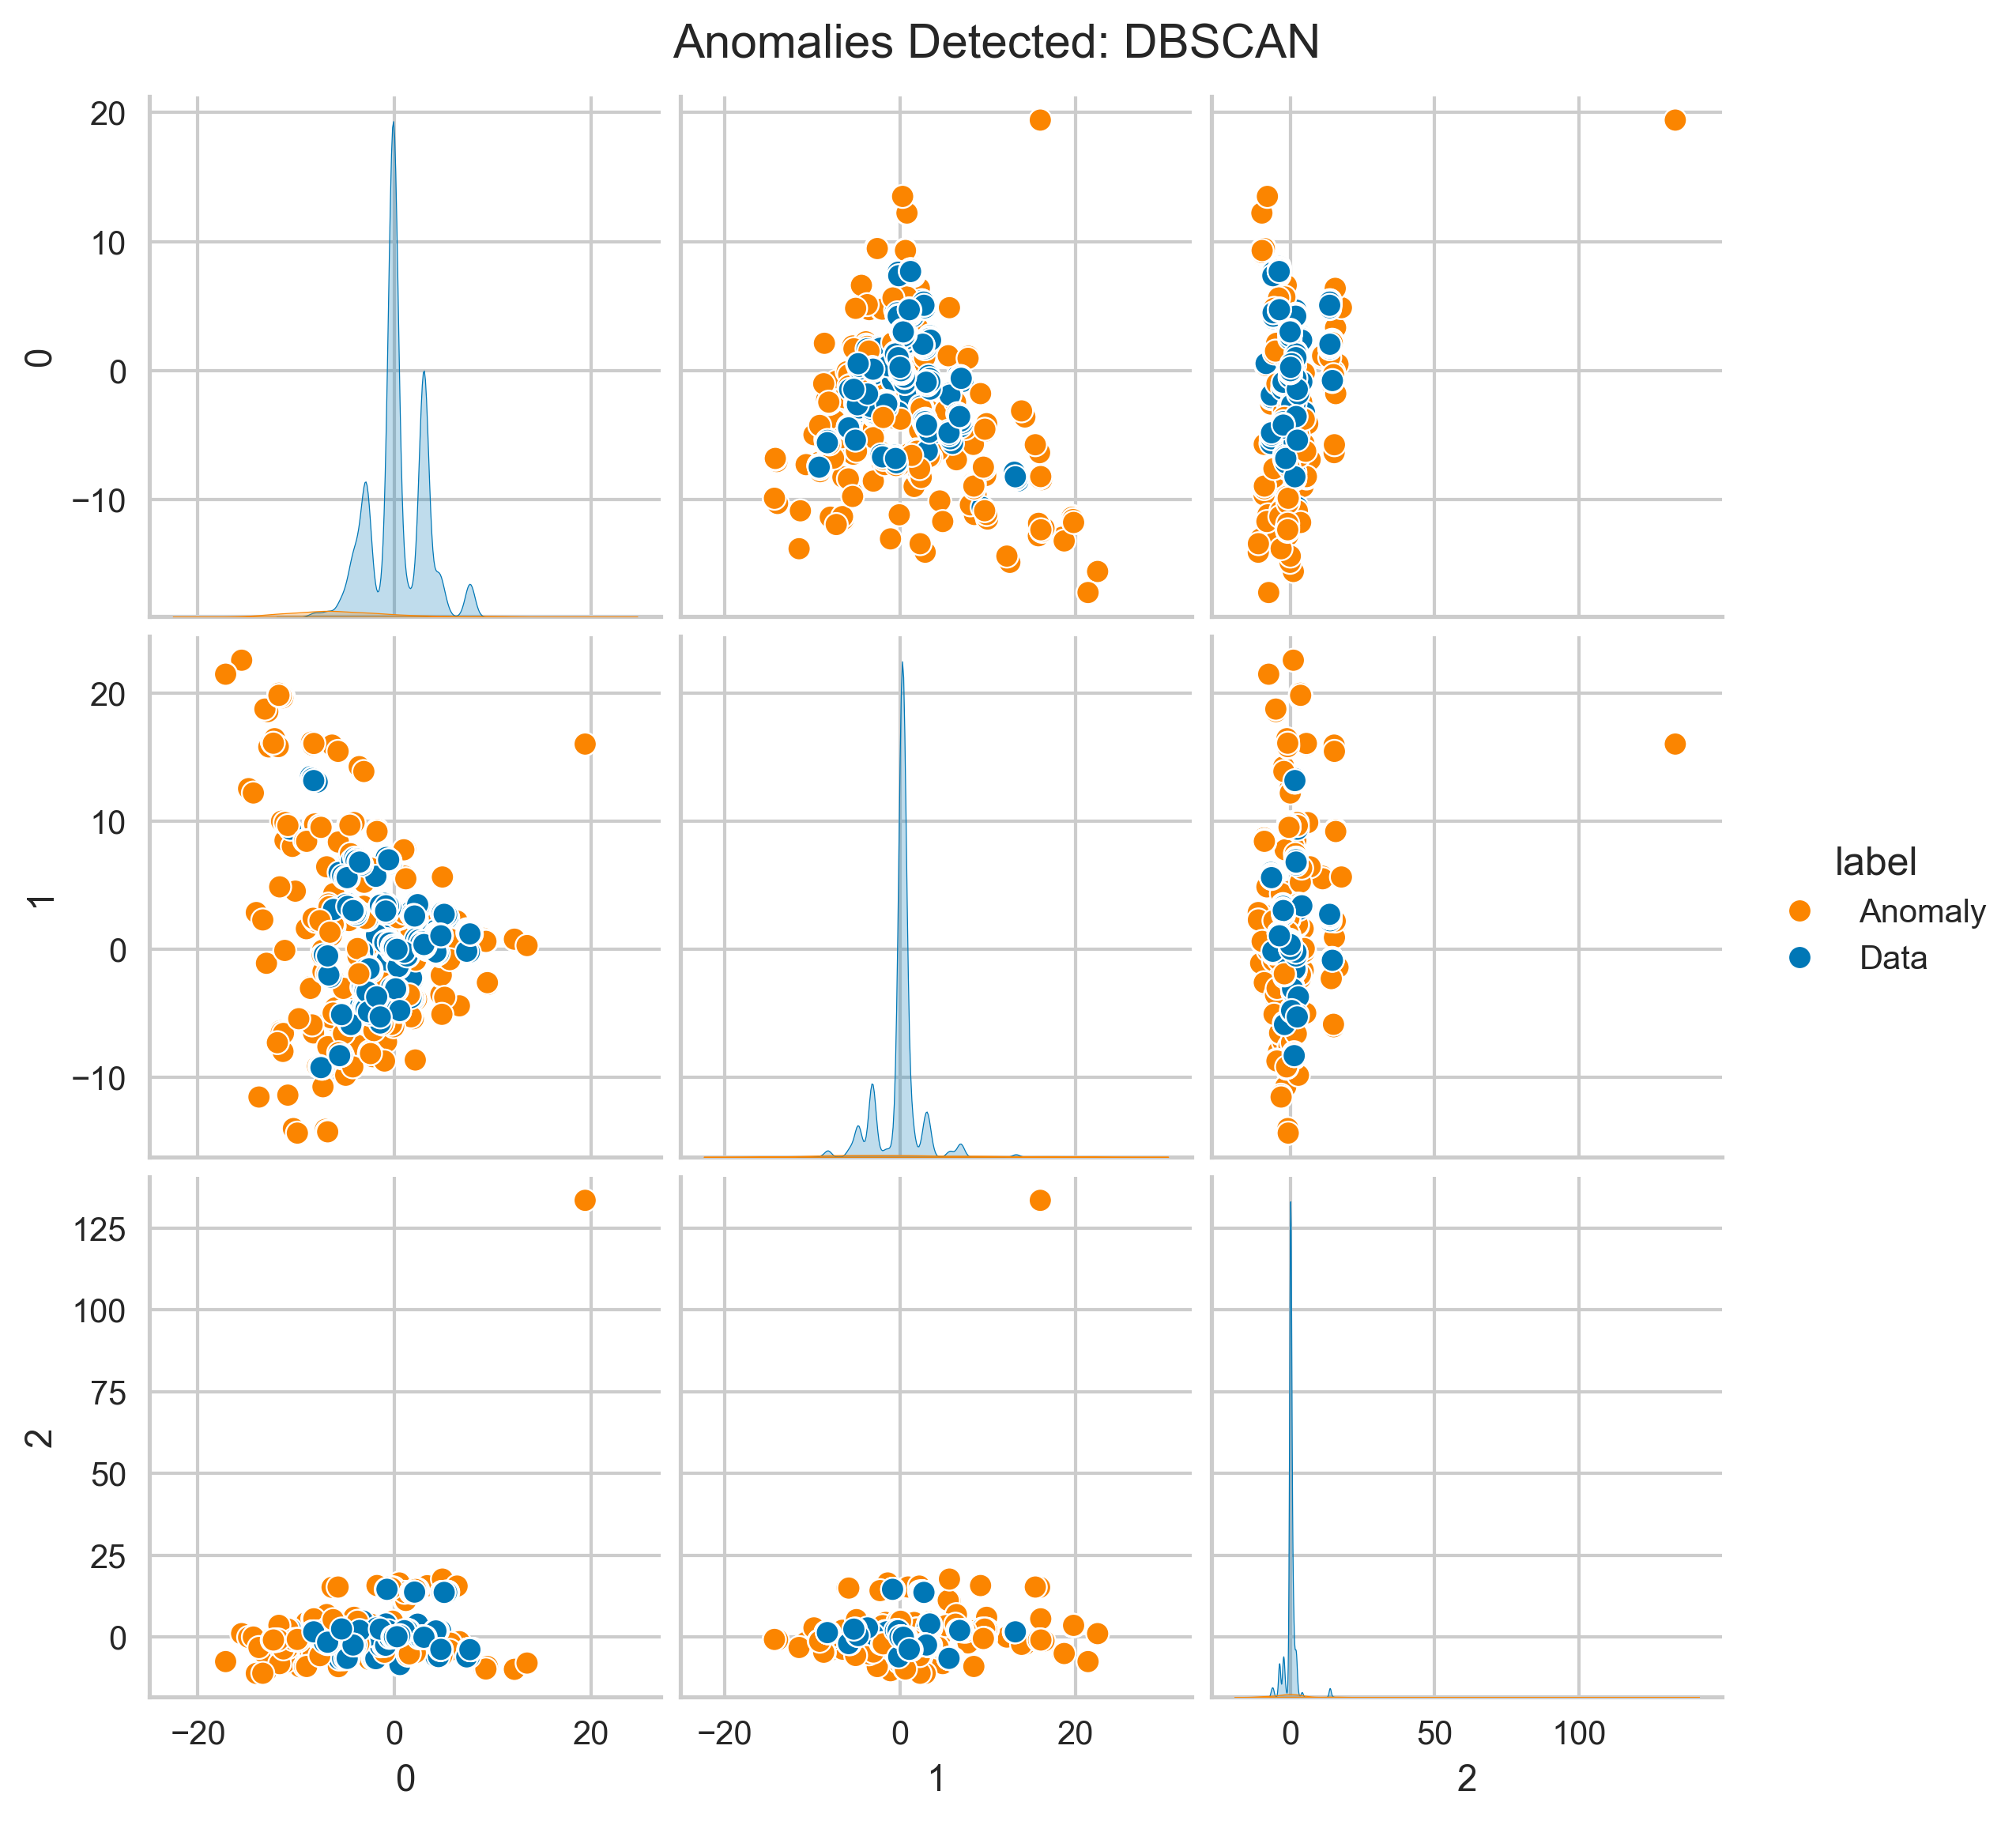
\includegraphics[width=0.45\textwidth]{images/famd_dbscan.png}
    \caption{Anomalies detected by DBSCAN with $\epsilon$ 0.035, Silhouette score 0.559 and 645 outliers visualized on the 3 coordinates of FAMD.}
    \label{fig:famd_dbscan}
\end{figure}

\subsection{HDBSCAN: LO METTIAMO???}

\section{Local Outlier Factor}
Local Outlier Factor (LOF) measures the local density deviation of a data point relative to its neighbors. Unlike global outlier detection methods, LOF considers the local context of each data point, making it robust to variations in data density. The algorithm assigns an outlier score to each data point, indicating its deviation from the local density of its neighbors. A high LOF score signifies a data point that is significantly less dense than its neighbors, thus classifying it as an outlier. \newline
As with the previous approaches, we calculated the Local Outlier Factor (LOF) using a precomputed proximity matrix. In our case, this matrix corresponds to the proximity matrix generated using the Gower distance.

\section{Comparison}
Different approches has been developed to address the problem of identifying outliers, here's is an overview of the performances for each kind of algorithms employed in this report. The performance metrics considered will take into consideration the number of anomalies identified but each algorithms and some metrics to evaluate the result of clustering algorithms, like for example the rand index. 

\subsection{Rand Index}

\section{Conclusions}
\begin{itemize}
    \item Summary of findings from different clustering methods
    \item Comparison of the effectiveness of each method for anomaly detection
    \item Implications for healthcare datasets and potential real-world applications
    \item Future work and improvements
\end{itemize}

\begin{thebibliography}{Com79}

\bibitem[Sander et al. 1998]{Sander-etal98}
J{\"o}rg Sander, Martin Ester, Hans-Peter Kriegel, and Xiaowei Xu.
\newblock \emph{Density-Based Clustering in Spatial Databases: The Algorithm GDBSCAN and Its Applications}.
\newblock \emph{Data Mining and Knowledge Discovery}, 2:169--194, 1998.

\end{thebibliography}

\end{document}




